\documentclass[11pt,landscape,a4paper,fleqn]{article}
\usepackage[utf8]{inputenc}
\usepackage[ngerman]{babel}
\usepackage{tikz}
\usetikzlibrary{shapes,positioning,arrows,fit,calc,graphs,graphs.standard}
\usepackage[nosf]{kpfonts}
\usepackage[t1]{sourcesanspro}
\usepackage{multicol}
\usepackage{wrapfig}
\usepackage[top=0mm,bottom=3mm,left=1mm,right=1mm]{geometry}
\usepackage[framemethod=tikz]{mdframed}
\usepackage{microtype}
\usepackage{mathtools}
\usepackage{ccicons}
\usepackage{hyperref}
\usepackage{xcolor}
\usepackage{soul}
\usepackage{amssymb}
\usepackage[neveradjust]{paralist}
\usepackage[shortlabels]{enumitem}
\usepackage{bbm}
\usepackage{listings}
\usepackage{titlesec}
\usepackage{anyfontsize}
\usepackage{nicefrac}
\usepackage{scalerel}
\usepackage{datatool}
\usepackage{amsmath}
\usepackage{amsfonts}
\usepackage{bbm}
\usepackage{bm}
\usepackage{ragged2e}
\usepackage{blindtext}
% \usepackage[x11names]{xcolor}


% \newcommand\hmmax{0}
% \newcommand\bmmax{0}


%fonts:
%\usepackage[nosf]{kpfonts}


%\usepackage[lf]{MyriadPro}
%\usepackage[lf,minionint]{MinionPro}

%\usepackage{mathptmx}
%\usepackage{cm}


\usepackage{paralist}
\usepackage[framemethod=tikz]{mdframed}
%Commands
\newcommand{\y}{\mathbf{y}}
\newcommand{\x}{\mathbf{x}}
\newcommand{\z}{\mathbf{z}}
\newcommand{\w}{\mathbf{w}}
\newcommand{\Z}{\mathcal{Z}}
\newcommand{\X}{\mathbf{X}}
\newcommand{\Y}{\mathbf{Y}}
\newcommand{\I}{\mathbf{I}}
\newcommand{\B}{\mathbf{B}}
\newcommand{\N}{\mathcal{N}}
\newcommand{\E}{\mathbb{E}}
\newcommand{\Prob}{\mathrm{\textbf{P}}}
\newcommand{\V}{\mathbb{V}}
\newcommand{\C}{\mathbb{C}}
\newcommand{\R}[0]{\mathbb{R}}
\DeclareMathOperator*{\argmin}{arg\,min}
\DeclareMathOperator*{\argmax}{arg\,max}

%Maps to with text on top%
\makeatletter
\newcommand{\xMapsto}[2][]{\ext@arrow 0599{\Mapstofill@}{#1}{#2}}
\def\Mapstofill@{\arrowfill@{\Mapstochar\Relbar}\Relbar\Rightarrow}
\makeatother

\endinput

\thinmuskip=1mu
\medmuskip=1mu %plus 2mu minus 4mu
\thickmuskip=1mu
\let\bar\overline

%\definecolor{mygrey}{cmyk}{0,0,0,0.8}
\definecolor{mathColor}{cmyk}{0,0,0,0.9}

\definecolor{sectionColor}{HTML}{4B0082}
\definecolor{subsectionColor}{HTML}{3364FF}

\definecolor{myorange}{cmyk}{0,0.5,1,0}
\definecolor{myorange2}{cmyk}{0,0.8,0.8,0}
\definecolor{darkgreen}{HTML}{4B0082}
\definecolor{mypink}{cmyk}{0, 0.7808, 0.4429, 0.1412}


% \DeclareMathOperator{\di}{d\!}
% \DeclareMathAlphabet{\mathcal}{OMS}{cmsy}{}{n}

\pgfdeclarelayer{background}
\pgfsetlayers{background,main}

\everymath\expandafter{\the\everymath \color{mathColor}}
\everydisplay\expandafter{\the\everydisplay \color{mathColor}}

\renewcommand{\baselinestretch}{.75}
\pagestyle{empty}


\makeatletter
\renewcommand{\section}{\@startsection{section}{1}{0mm}%
                                {.2ex}%
                                {.2ex}%x
                                {\color{sectionColor}\sffamily\small\bfseries}}
                                

%Firebrick1
\renewcommand{\subsection}{\@startsection{subsection}{1}{0mm}%
                                {.2ex}%
                                {-1ex}%x
                                {\color{subsectionColor}\sffamily\bfseries}}

% \usepackage{titlesec}
% \titlespacing*{\subsubsection}{0pt}{-2pt}{-6pt}


\makeatother
\setlength{\parindent}{0pt}
\setlength{\columnsep}{5pt}

\begin{document}
\small
\begin{multicols*}{4}
\fontdimen2\font=0.25ex
% \section*{Introduction}
\subsection*{Prob. Basics} \;
\textbf{Normalization}: \; $P(\Omega) = 1$ \\
\textbf{Non-neg}: \; $\forall A \in \mathcal{F}, P(A) \geq 0$ \;
\textbf{$\sigma$-add:} \; $\forall A_{1},..., A_{n} \in \mathcal{F}$ 

\textbf{Disjoint}: \; $P \left(\bigcup\limits_{i=1}^{\infty} A_{i} \right) = \sum\limits_{i=1}^{\infty}P(A_{i})$

\textbf{Conditional probability}: \; $P(X|Y)$

\textbf{Prod. Rule}: \; $P(X,Y)=P(X|Y)P(Y)=P(Y|X)P(X)$

\textbf{Chain (Joint Prob.)}: \; $P(X_1, ..., X_n) = P(X_{1:n})$ \\
$=P(X_1)P(X_2|X_1)P(X_3|X_{1:2})...P(X_n|X_{1:n-1})$

\textbf{Sum (Joint Prob.)}: \; $P(X_{1:n}) = \sum_y P(X_{1:n}, Y=y)$ \\
\; \; $=\sum_y P(X_{1:n}|Y=y)P(Y=y)$ \\
\; \; $=\int_y P(X_{1:n}|Y=y)P(Y=y)dy$

\vspace*{-1mm}
\textbf{Bayes' Rule:} \; $P(X|Y) = \frac{P(X,Y)}{P(Y)} = \frac{P(Y|X)P(X)}{P(Y)}$

\textbf{X, Y indep.:} \; $P(X|Y) = P(X)$, \;$P(X,Y) = P(X) P(Y)$

\textbf{Exp:} \; $\mathbb{E}_x[f(X)] = \int f(x)p(x)dx = \sum_x f(x)p(x)$

\textbf{Lin. Exp:} \; $\mathbb{E}_{x,y}[aX + bY] = a\mathbb{E}_x[X] + b \mathbb{E}_y[Y]$

\textbf{Var:} \; $Var[X] = \mathbb{E}[(X-\mu_X)^2] = \mathbb{E}[X^2] - \mathbb{E}[X]^2$

$Var(X + Y) = Var(X) + Var(Y) + 2Cov(X,Y)$

\textbf{Cov:} \; $Cov(X, Y) = \mathbb{E}[(X - \mathbb{E}[X])(Y - \mathbb{E}[Y])]$

\textbf{CoV:} \; $Y = g(X)$, $f_Y(y) = f_X(g^{-1}(y)) \cdot |\frac{d}{dy} g^{-1}(y)|$

\vspace*{-0.5mm}
\textbf{Gauss:} \; \mbox{\fontsize{8}{6}\selectfont $\mathcal{N} = \left(\nicefrac{1}{\sqrt{(2\pi)^d |\Sigma|}}\right) exp(-\frac{1}{2}(x-\mu)^T\Sigma^{-1} (x-\mu))$}

\vspace*{-0.5mm}
\textbf{CDF:} \; \mbox{\fontsize{9}{6}\selectfont $\Phi(u;\mu,\sigma^2) = \int_{-\infty}^{u}\mathcal{N}(y;\mu,\sigma^2)dy=\Phi(\frac{u-\mu}{\sqrt{\sigma^2}};0,1)$;}

\vspace*{-0.5mm}
\textbf{Multivar. Gauss:} \;
\mbox{\fontsize{8}{6}\selectfont $X_V = [X_1, .., X_d] \sim \mathcal{N}(\mu_V, \Sigma_{VV})$},

index sets \mbox{\fontsize{8}{6}\selectfont $A = \{i_1,..,i_k\}$, $B = \{j_1,..,j_m\}$, $A \cap B = \emptyset$}

\textbf{Marginal:} \; \mhl{$X_A = [X_{i_1},..X_{i_k}] \sim \mathcal{N}(\mu_A, \Sigma_{AA})$} with \\
\mbox{\fontsize{8.8}{6}\selectfont $\mu_A = [\mu_{i_1},..,\mu_{i_k}]$},
\mbox{$\Sigma_{AA}^{(m,n)} = \sigma_{i_m,i_n} = \mathbb{E}[(x_{i_m} - \mu_{i_m}) (x_{i_n} - \mu_{i_n})]$}

\textbf{Cond2DisjSets:} \; $P(X_A | X_B = x_B) = \mathcal{N}(\mu_{A|B}, \Sigma_{A|B})$, \\ 
\mhl{$\mu_{A|B} = \mu_A + \Sigma_{AB} \Sigma_{BB}^{-1} (x_B - \mu_B)$}, \\ 
\mhl{$\Sigma_{A|B} = \Sigma_{AA} - \Sigma_{AB} \Sigma_{BB}^{-1} \Sigma_{BA}$}

$Y = M X_A, M \in \mathbb{R}^{m \times d}$, \hfill \mhl{$Y \sim \mathcal{N}(M\mu_A, M\Sigma_{AA}M^T)$} \;

$Y = X_A + X_B$, \hfill \mhl{$Y \sim \mathcal{N}(\mu_A + \mu_B, \Sigma_{AA} + \Sigma_{BB})$} \;

%-------------------------------------------------------------------------------------------
%Calculus and stuff
%-------------------------------------------------------------------------------------------

%$ln(x) \leq x - 1, x>0$; $||x||_2 = \sqrt{x^T x}$; $\nabla_x ||x||_2^2 = 2 x$%; $||x||_p = (\sum_{i=1}^n|x_i|^p)^{\frac{1}{p}}$, $1 \leq p < \infty$

% KL divergence

\textbf{KL}: \;
\mhl{$KL(p||q) = \mathbb{E}_p[log\frac{p(x)}{q(x)}] = \sum_{x \in X} p(x) \cdot log \frac{p(x)}{q(x)}$} \\
\vspace*{-0.5mm}
\mhl{$= \int p(x) log \frac{p(x)}{q(x)} \, dx \geq 0$}, \; $p=q \rightarrow KL(p||q) = 0$

% Entropy
\textbf{Entropy}: \; \mhl{{\fontsize{9.5}{6}\selectfont $H(q) = \mathbb{E}_q[-\log q(\theta)] = - \int q(\theta)\log q(\theta) d\theta $}}

\mhl{$=- \sum_\theta q(\theta) \log q(\theta)$}; \;
$H(\prod q_i(\theta_i)) = \sum_i H(q_i)$; \\
$H(N(\mu, \Sigma)) = \frac{1}{2}  ln|2\pi e \Sigma|$; $H(p,q) = H(p) + H(q | p)$

$H(S | T) \geq H(S | T, U)$ \textit{'information never hurts'}

\textbf{Orth:} \; A: $A^{-1}=A^T,AA^T=A^TA=||A||_2^2=I$\\
$det(A)\in\{+1,-1\}, (A^{-1})^T=(A^T)^{-1}, rank(A)=n$

\textbf{Inv:} \; $A^{-1}=
\big[
\begin{smallmatrix}
a&b \\ 
c&d
\end{smallmatrix}\big]^{-1}=
\frac{1}{ad-bc}
\big[
\begin{smallmatrix}
d&-b \\ 
-c&a
\end{smallmatrix}\big];
$

\textbf{Deriv:} \;
$(fg)' = f'g + fg'$; $(f/g)' = (f'g - fg')/g^2$

$f(g(x))' = f'(g(x))g'(x)$; $\log(x)' = 1/x$
%$\frac{\partial}{\partial x}b^Tx=\frac{\partial}{\partial x}x^Tb=b,\!
%\frac{\partial}{\partial x}x^Tx=\frac{\partial}{\partial x}||x||_2^2=2x,\!
%\frac{\partial}{\partial x}(x^TAx)=(A^T+A)x,$
%$\frac{\partial}{\partial x}(b^TAx)=A^Tb, \frac{\partial}{\partial X}(c^TXb)=c^Tb,
%\frac{\partial}{\partial X}(c^TX^Tb)=bc^T$

\iffalse
\textbf{Eigdec:} \;
$A,Q \in \mathbb{R}^{n\times n}, A=Q\Lambda Q^{-1},\! \Lambda = diag(\lambda_i)$\\
$Q=[v_1,..,v_n], \text{(col's are e-vec.)}$

if all $\lambda_i\geq0: A^{-1}=Q\Lambda^{-1}Q^{-1},\Lambda^{-1}=diag(\frac{1}{\lambda_i})$\\
if $A=A^T\text{(symm.) and }x^TAx\geq0 \forall x \neq 0 \rightarrow psd$

\textbf{SVD:} \;
$X\in \mathbb{R}^{n\times p}, U\in \mathbb{R}^{n\times n}, S\in \mathbb{R}^{n\times p},
V\in \mathbb{R}^{p\times p}$\\
$X=USV^T=\sum_{k=1}^{rank(X)}\sigma_{k,k}u_k (v_k)^T,\!${\tiny{($U^TU=V^TV=I$)}}\\
$X^TX=VS^TU^TUSV^T=VS^TSV^T=V\Sigma V^T$\\
$\Sigma = diag(\sigma_1^2,..,\sigma_n^2);\sigma_i^2=\lambda_i; \forall \lambda_i \geq 0$
\fi



%CDF: cumulative distribution function; PDF: standard normal probability density function, $\mu = 0$, $\sigma = 1$
%PDF: $\phi(x) = \frac{1}{\sqrt{2\pi}} e^{-(1/2)x^2}$; $\int \phi(x) \partial x = \Phi(x) + c$;\\
%$\int x \phi(x) = -\phi(x) + c$; $\int x^2 \phi(x) \partial x = \Phi(x) -x \phi(x) + c$

\textbf{Cnvx:} \; $\text{g(x) convex} \Leftrightarrow x_1,x_2 \in \mathbb{R}, \lambda \in [0,1]: g\text{''}(x) > 0$; \\ 
\hfill $g(\lambda x_1 + (1-\lambda) x_2) \leq \lambda g(x_1) + (1-\lambda) g(x_2)$

\mhl{\textbf{Jensen ineq.:} \; $g$ convex: $g(E[X]) \leq E[g(X)]$}

\mhl{$g$ concave (e.g. $\log$): $g(E[X]) \geq E[g(X)]$}

\subsection*{Bayesian Learning} \;
\textbf{Prior:} \; $p(\theta)$;

\textbf{Likelihood:} \; $p(y_{1:n} | x_{1:n}, \theta) = \prod_{i=1}^{n} p(y_i | x_i, \theta)$;

\textbf{Posterior} \; $p(\theta | x_{1:n}, y_{1:n}) = \frac{1}{Z} p(\theta) \prod_{i=1}^{n} p(y_i | x_i, \theta)$;

where $Z = \int p(\theta) \prod_{i=1}^{n} p(y_i | x_i, \theta) d\theta$ (norm. const.);

\textbf{P:} \; $p(y^* | x^*, x_{1:n}, y_{1:n}) = \int p(y^* | x^*, \theta) p(\theta | x_{1:n}, y_{1:n}) d\theta$

\subsection*{Bayesian Lin. Reg.}
\textbf{Prior:} \; $p(\mathbf{w}) = \mathcal{N}(0, \sigma_w^2 \mathbf{I})$, \\ 
\textbf{Likelihood:} \; $p(y_i|\mathbf{x_i}, \mathbf{w}, \sigma_n) = \mathcal{N}(y_i; \mathbf{w}^T\mathbf{x_i}, \sigma_n^2)$ \\
\textbf{Posterior:} \; $p(\mathbf{w} | \mathbf{X, y}) = \mathcal{N}(\mathbf{w}; \overline{\mu}, \overline{\Sigma})$, \\
\mhl{$\overline{\Sigma} = (\sigma_n^{-2}\mathbf{X}^T\mathbf{X} + \sigma_w^{-2} \mathbf{I})^{-1}$,
$\overline{\mu} = \sigma_n^{-2} \overline{\Sigma} \mathbf{X}^T\mathbf{y}$}; \\
$p(f^* | \mathbf{X,y,x^{*}}) = \mathcal{N}(\mathbf{x^*}^T\overline{\mu}, {\mathbf{x}^*}^T \overline{\Sigma} \mathbf{x}^{*})$; \\
$p(y^* | \mathbf{X,y,x^{*}}) = \mathcal{N}({\mathbf{x}^{*}}^T \overline{\mu}, \textcolor{red}{{\mathbf{x}^{*}}^T \overline{\Sigma} \mathbf{x}^*} + \textcolor{orange}{\sigma_n^2})$

\textcolor{red}{\textbf{Epistemic}}: uncertainty about model due to lack of data. \; \textcolor{orange}{\textbf{Aleatoric:}} Irreducible noise

\textbf{Recursive updates:} \\ $\mathbf{X}_{t+1}^T \mathbf{X}_{t+1} = \mathbf{X}_{t}^T \mathbf{X}_{t} + x_{t+1} x_{t+1}^T$

$\mathbf{X}_{t+1}^T y_{t+1} = \mathbf{X}_{t}^T y_{t} + y_{t+1} x_{t+1}$

\textbf{Parallel to Ridge Reg.: } \;
$f(x,w) = y \approx \mathbf{w}^\top \mathbf{x}$ \\ 
$\hat{w} = \arg\min_{w}\sum_{i=1}^{n}(y_i - w^\top x_i)^2 + \lambda \|w\|_2^2$ \\ 
$= (X^{\top} X + \lambda I)^{-1}X^{\top} y \rightarrow$ MAP Bayesian inf. w/\\
$p(w) = N(0, \sigma_p^2 I)$ and $\epsilon_i \sim N(0, \sigma_n^2)$, then $\lambda = \nicefrac{\sigma_n^2}{\sigma_p^2}$ \\
$f^{*} = \mathbf{w}^T\mathbf{x}^{*}$, $y^{*} = f^{*} + \epsilon$, $\epsilon \sim \mathcal{N}(0, \sigma_y^2)$

\vspace*{-0.8mm}
\subsection*{BLogR:} \; $p(y_i | x_i, \theta) = \sigma(y_i w^T x_i)$, \; $\sigma(a) = \frac{1}{1 + e^{-a}}$

\subsection*{Kalman Fil:} $X_{t+1} \bot X_{1:t-1} | X_t, Y_t \bot Y_{1:t-1}, X_{1:t-1} | X_t$,

State $X_t$, Observation $Y_t$, Prior $P(X_1)  \sim \mathcal{N}(\mu, \Sigma)$

Motion model: $P(\mathbf{X}_{t+1} | \mathbf{X}_t) = \mathcal{N}(x_{t+1}; \mathbf{F} X_t, \Sigma_x)$, \mhl{$\mathbf{X}_{t+1} = \mathbf{F} \mathbf{X}_{t} + \epsilon_t$, $\epsilon_t \sim \mathcal{N}(0, \Sigma_x)$}

Sensor model: \hfill $P(\mathbf{Y}_t | \mathbf{X}_t) = \mathcal{N}(y_t; H X_t, \Sigma_y)$, \mhl{$\mathbf{Y}_t = \mathbf{H} \mathbf{X}_t + \eta_t$, $\eta_t \sim \mathcal{N}(0, \Sigma_y)$}

\textbf{Kalman Gain:} \;
\mhl{$\mathbf{K}_{t+1} = ( \mathbf{F} \Sigma_t \mathbf{F}^T + \Sigma_x ) \cdot $}\\ 
\mhl{$\cdot \mathbf{H}^T ( \mathbf{H} (\mathbf{F} \Sigma_t \mathbf{F}^T + \Sigma_x ) \mathbf{H}^T + \Sigma_y )^{-1}$}

\textbf{Kalman Update:} \\
$\mu_{t+1} = \mathbf{F} \mu_t + \mathbf{K}_{t+1} (\mathbf{y}_{t+1} - \mathbf{H} \mathbf{F} \mu_t)$

$\Sigma_{t+1} = (\mathbf{I} - \mathbf{K}_{t+1} \mathbf{H}) (\mathbf{F} \Sigma_t \mathbf{F}^T + \Sigma_x)$

\textbf{Bayesian Filtering in KFs} \\
Keep track of state $X_t$ using rec. formula. \\
Start $P(X_1) = \mathcal{N}(\mu, \Sigma)$. \\
At time $t$: assume we have $P(X_t | y_{1:t-1})$

\textbf{Conditioning:} \; \mhl{$P(X_t | y_{1:t}) = \frac{1}{Z} P(y_t | X_t) P(X_t | y_{1:t-1})$}

\textbf{Prediction:} \;\mhl{$P(X_{t+1} | y_{1:t}) = \int \hspace*{-1mm} P(X_{t+1} | x_t) P(x_t | y_{1:t}) dx_t$}

\vspace*{-0.5mm}
\subsection*{Gaussian Processes}

Gaussian distr. over functions $f \sim GP(\mu(x),K(x))$ ($\infty$-d Gaussian). 

Infinite set of RVs $X$ s.t. $\forall A \subseteq X, A = \{ x_1,.., x_m\}$
it holds \mhl{$Y_A = [Y_{x_1},..,Y_{x_m}] \sim \mathcal{N}(\mu_A, K_{AA})$} where

$K_{AA}^{(ij)} = k(x_i, x_j)$ and $\mu_A^{(i)} = \mu(x_i)$ with covariance (kernel) function $k(\cdot, \cdot)$, mean function $\mu(\cdot)$

\textbf{Cov. (Kernel)} $k$: \; symmetric, PSD, kernel composition rules hold,
%$k(x,x') = k_1(x,x') + k_2(x,x')$, $k(x,x') = k_1(x,x') \cdot k_2(x,x')$, $k(x,x') = c \cdot k_1(x,x'), c > 0$, $k(x,x') = f(k_1(x,x'))$, $f$: polynomial with coeffs $> 0$ or $f(x) = e^x$,
stationary: $k(x,x') = k(x - x')$,

isotropic: $k(x,x') = k(||x - x'||_2)$.

\textbf{GP Pred:} \; $p(f|x_{1:m},y_{1:m}) = GP(f; \mu(x), k(x,x'))$, 

observe $y_i = f(x_i) + \epsilon_i$, $\epsilon_i \sim \mathcal{N}(0, \sigma^2)$, \mbox{\fontsize{9}{6}\selectfont $A = \{x_1,..,x_m\}$}.

Common convention: prior mean $\mu(x) = 0$

Then \mhl{$p(f | x_{1:m}, y_{1:m}) = GP(f; \mu', k')$} where

\mhl{$\mu'(x) = \mu(x) + \mathbf{k}_{x,A} (\mathbf{K}_{AA} + \sigma^2 \mathbf{I})^{-1} (\mathbf{y}_A - \mu_A)$} \\
\mhl{$k'(x,x') = k(x, x') - \mathbf{k}_{x,A} (\mathbf{K}_{AA} + \sigma^{2} \mathbf{I})^{-1} \mathbf{k}_{x',A}^T$}

$k_{x,A} = [k(x, x_1),..., k(x, x_m)]$

\textbf{Pred posterior:} \; $p(y^* | x_{1:m}, y_{1:m},x^*) = \mathcal{N}(\mu_y^*, {\sigma_y^2}^*)$, $\mu_y^* = \mu'(x^*)$, \; ${\sigma_y^2}^* = \sigma^2 + k'(x^*, x^*)$

\textbf{Forward sampling GP:} \; Chain rule on $P(f_1,..,f_n)$, iteratively sample univariate Gauss

\textbf{Model selection:} \; max. marginal likelihood

$\hat{\theta} = amax_\theta p(y | X, \theta) = amax_\theta \int p(y | X,f) p(f | \theta) df$

%\textbf{Model selection:} optimize marginal likelihood $p(y | X, \theta) = \int p(y | X,f) p(f | \theta) df$:

%$\hat{\theta} = amin_{\theta} -\log p(y | X, \theta) = amin_{\theta} \textcolor{red}{y^T K_y(\theta)^{-1} y +}$

%$\textcolor{red}{\log |K_y(\theta)|}$ $\rightarrow$ use GD $\theta^{t+1} \leftarrow \theta^t - \eta_t \nabla \textcolor{red}{L(\theta)}$

\textbf{Fast GPs}: GP prediction has cost $\mathcal{O}(|A|^3)$

1) \; Local: distance decaying kernel (e.g. RBF), only condition on points $x'$ where $|k(x,x')| \geq \tau$

2) \; $k$ low-d approx: $k(x,x') \approx \phi(x)^T \phi(x')$, then BLR

3) \; RFF: Stationary kernel has FT: \; \mhl{$k(x,x')$} 

$= \int_{\mathbb{R}^d} p(\omega) e^{j \omega^T (x - x')} d\omega = \mathbb{E}_{\omega, b}[z_{w,b}(x) z_{w,b}(x')]$ 

\mhl{$\approx \frac{1}{m} \sum_i z_{w^{(i)},b^{(i)}}(x) z_{w^{(i)},b^{(i)}}(x')$},

$\omega \sim p(\omega), b \sim \mathcal{U}[0, 2\pi], z_{\omega, b}(x) = \sqrt{2} \cos(\omega^T x + b)$

%$\rightarrow$ draw finitely many samples $\omega_i, b_i$

$\rightarrow$ $k(x,x') \approx \phi(x)^T \phi(x')$ ($\phi_i(x) = \frac{1}{\sqrt{m}} z_{w^{(i)},b^{(i)}}(x)$)

4) \; \textbf{Inducing Points Methods:} \; Sum. data via

values of $f$ at inducing points $\mathbf{u} = [u_1,..,u_m]$.

$p(f^*, f) = \int p(f^*, f, u) du = \int p(f^*, f | u) p(u) du$

$p(f^*, f) \approx q(f^*, f) = \int q(f^* | u) q(f | u) p(u) du$

with $p(f | u) = \mathcal{N}(K_{f,u} K_{u,u}^{-1} u, K_{f,f} - Q_{f,f} )$,

$p(f^* | u) = \mathcal{N}(K_{f^*,u} K_{u,u}^{-1} u, K_{f^*, f^*} - Q_{f^*, f^*})$,

and $Q_{a,b} = K_{a,u} K_{u,u}^{-1} K_{u,b}$, $p(\mathbf{u}) \sim \mathcal{N}(0, K_{u,u})$

\textbf{Subset of Regressors:} \; assume $K_{f,f} - Q_{f,f} = 0$,

replace $p(f|u)$ by $q_{\text{\tiny SoR}}(f|u) = \mathcal{N}(K_{f,u} K_{u,u}^{-1} u,0)$

resulting model is degenerate GP with covariance function $k_{SoR}(x,x') = k(x,u) K_{u,u}^{-1} k(u, x')$

\textbf{FITC:} \; Assume $f_i \indep f_j | u, \forall i \neq j$

\vspace*{-1mm}
$q_{FITC}(f | u) = \mathcal{N}(K_{f,u} K_{u,u}^{-1} u, diag(K_{f,f} - Q_{f,f}))$


% Laplace Approximation
\subsection*{Laplace Approx}
$p(w|(x,y)_{1:n}) \approx q_\lambda(\theta) = \mathcal{N}(\hat{\theta}, \Lambda^{-1})$

$\hat{\theta} = \arg\max_\theta p(\theta | y)$, $\Lambda = - \nabla\nabla \log p(\hat{\theta} | y)$

Predict: $p(y^*| x^*, x_{1:n}, y_{1:n}) \approx \int p(y^* | f^*) q(f^*) df^*$,

\vspace*{-1mm}
with $q(f^*) = \int p(f^* | \theta) q_\lambda(\theta) d\theta$.  LA first greedily fits mode, then matches curvature (over-conf.).

% Variational Inference
\subsection*{Variational Inf.} \;
$\textcolor{darkgreen}{p(\theta | y)} = \frac{1}{Z} p(\theta, y) \approx \textcolor{red}{q_\lambda(\theta)}$

$q_{bwd}^* \in \arg\min_{q \in \mathcal{Q}} KL(\textcolor{red}{q} || \textcolor{darkgreen}{p})$: \; $q \approx p$ where q large

$q_{fwd}^* \in \arg\min_{q \in \mathcal{Q}} KL(\textcolor{darkgreen}{p} || \textcolor{red}{q})$: \; $q \approx p$ where p large

\mhl{$amin_q KL(q||p) = amax_q \mathbb{E}_{\theta \sim q}[\log p(\theta, y)] + H(q(\theta))$}
\mhl{$ = amax_q \mathbb{E}_{\theta \sim q}[\log p(y | \theta)] - KL(q(\theta)||p(\theta))$}

\textbf{ELBO:} \; $L(q) = \mathbb{E}_{\theta \sim q} [\log p(y, \theta)] + H(q) \leq \log p(y)$

\textbf{NOTE:} \; $q( \cdot | \lambda)$ dep. on var. params, ELBO then 

\textbf{ELBO$_{\lambda}$:} \; $ L(\lambda) = \mathbb{E}_{\theta \sim q(\cdot | \lambda)} [\log p(y | \theta)] - KL(q_{\lambda} || p(\cdot))$

 $\rightarrow$ $\nabla_\lambda L(\lambda)$ tricky due to  $\textcolor{red}{\theta \sim q_\lambda(\cdot)}$

\textbf{Reparametrization Trick:} \; Suppose $\epsilon \sim \phi$, 

\vspace*{-1mm}
$\theta = g(\epsilon, \lambda)$. Then: $q(\theta | \lambda) = \phi(\epsilon) |\nabla_\epsilon g(\epsilon; \lambda)|^{-1}$ (CoV) 

and \mhl{$\mathbb{E}_{\theta \sim q_\lambda}[f(\theta)] = \mathbb{E}_{\epsilon \sim \phi}[f(g(\epsilon; \lambda))]$}, which allows 

\mhl{$\nabla_\lambda \mathbb{E}_{\theta \sim q_\lambda}[f(\theta)] = \mathbb{E}_{\epsilon \sim \phi}[\nabla_\lambda f(g(\epsilon; \lambda))]$}


\subsection*{Markov Chains} 
A \mhl{stationary MC} is a sequence of RVs $X_1,..,X_N$ with prior $P(X_1)$ and transition probability $P(X_{t+1} | X_t)$ independent of $t$. 
An \mhl{ergodic MC} if $\exists$ $t < \infty$ s.t. every state is reachable from every state in \textit{exactly} $t$ steps.

\textbf{Markovian Assumption:} \; $X_{t+1} \indep X_{1:t-1} | X_t \, \forall t$

\textbf{Stationary Distribution:} \; A stationary ergodic MC has a unique and positive stationary distr. $\pi(X) > 0$ s.t. \mhl{$\forall x$: $\lim_{N \rightarrow \infty} P(X_N = x) = \pi(x)$} and $\pi(X)$ is independent of prior $P(X_1)$.

Simulate MC via forward sampling (chain rule)

\vspace*{-0.5mm}
\subsection*{MCMC} Approx pred. distr. \mhl{$p(y^* | x^*, x_{1:n}, y_{1:n}) =$}

\vspace*{-0.5mm}
$\int \textcolor{darkgreen}{p(y^* | x^*, \theta)} p(\theta | (x,y)_{1:n})d\theta = \mathbb{E}_{\theta \sim p(\cdot | (x,y)_{1:n})}[\textcolor{darkgreen}{f(\theta)}]$

\vspace*{-0.5mm}
\mhl{$\approx \frac{1}{m} \sum_{i=1}^{m} f(\theta^{(i)})$}, sample $\theta^{(i)} \sim p(\theta | (x,y)_{1:n})$ from MC with stationary distribution $p(\theta| (x,y)_{1:n})$.

\textbf{Hoeffding:} \; ($P(err) \searrow$ exp.) Assume $f \in [0,C]$:

\mbox{\fontsize{9.5}{6}\selectfont $P(|\mathbb{E}_P[f(X)] - \frac{1}{N}\sum_{i=1}^{N} f(x_i)| > \epsilon) \leq 2 exp(-2N\epsilon^2/C^2)$}

Given unnormalized distr. $Q(x) > 0$, design MC s.t. $\pi(x) = \frac{1}{Z} Q(x)$. If MC satisfies \textbf{detailed\\ balance equation (DBE)} $\forall x,x'$:

\vspace*{-0.5mm}
\mhl{$Q(x)P(x' | x) = Q(x')P(x | x')$} $\implies$ $\pi(x) = \frac{1}{Z} Q(x)$.

\textbf{Gibbs Sampling:} \; Asympt. correct but slow

1. Init $\mathbf{x^{(0)}}$, fix observed RVs $X_B$ to $\mathbf{x_B}$\\
2. Repeat: set $\mathbf{x}^{(t)} = \mathbf{x}^{(t-1)}$; \textcolor{red}{select} $\textcolor{red}{j \in \{1:m\} \setminus B}$\\
$x_j^{(t)} \sim P \left(X_j | \mathbf{x}^{(t)}_{\{1:m\} \setminus \{j\}}\right)$ (efficient samples)

\vspace*{-0.5mm}
\textcolor{red}{Random Order:} \; fulfills DBE, find correct distr.

\textcolor{red}{Determ. Order:} \; not fulfill DBE, still correct distr.

\textbf{Expectations via MCMC:} \; Use MCMC sampler (e.g. GS) to get samples $\mathbf{X}^{(1:T)}$. After burn-in time $t_0$: \;
\mhl{$\mathbb{E}[f(\mathbf{X}) | \mathbf{x}_b] \approx \frac{1}{T - t_0} \sum_{\tau = t_0 + 1}^{T} f(\mathbf{X}^{(\tau)})$}

\textbf{Metropolis/Hastings:} \; Generate MC s.t. DBE sat.

1) Prop. $R(X' | X)$, $X_t = x$, sample $x' \sim R(X' | X=x)$; 
2) For $X_t = x$, w.p. \mhl{$\alpha =\min \{ 1, \frac{Q(x')R(x | x')}{Q(x) R(x' | x)}\}$}: $X_{t+1} = x'$; w.p. $1 - \alpha$: $X_{t+1} = x$

% p(x) is log-concave if f is convex
\vspace*{-0.5mm}
Cont RV: log-concave $p(x) = \frac{1}{Z} exp(-f(x))$, $f$ cnvx \\
M/H: \; $\alpha = \min \{ 1, \frac{R(x|x')}{R(x'|x)}exp(f(x) - f(x')\}$

\vspace*{-0.5mm}
MALA/LMC: \; $R(x' | x) = \mathcal{N}(x'; x - \tau \nabla f(x); 2\tau I)$

$\rightarrow$ Use gradient information for convergence

\subsection*{BNN} Prior NN $\theta$; NN parametrizes likelihood

$\mu$ \& log $\sigma^{2}$: \; $p(y|\mathbf{x}, \theta ) = \mathcal{N}(y;f_{1}(\mathbf{x}, \theta), exp(f_{2}(\mathbf{x}, \theta)))$

\vspace*{-0.5mm}
MAP/SGD: $\hat{\theta} = amin_\theta - \log p(\theta) - \sum_{i} \log p(y_i | x_i, \theta)$

$\rightarrow$ Handles heteroscedastic noise well, fails to \\
predict epistemic uncertainty $\rightarrow$ use VI

\vspace*{-0.5mm}
\textbf{VI(BbB):} \; SGD-opt ELBO via $\nabla_\lambda L(\lambda)$. Find VI \\
approx $q_\lambda$. Draw $m$ weights $\theta^{(j)} \sim q_\lambda(\cdot)$. Predict \mhl{$p(y^* | x^*, x_{1:n}, y_{1:n}) \approx \frac{1}{m} \sum_j p(y^* | x^*, \theta^{(j)})$}

\vspace*{-0.5mm}
\textbf{MCMC:} \; Produce seq. of weights {\fontsize{9}{6}\selectfont $\theta^{(1)},..,\theta^{(T)}$} via SGLD, LD, SG-HMC; predict by avg. weights.

%Summarize $\theta^{(i)}$ by subsampling or Gaussian approx.
\subsection*{Active Learning}

%Collect data that maximally reduces uncertainty.
\mbox{Pick $x$ max. reduce uncertainty}

\textbf{Mutual Info:} \; \mhl{$I(X;Y) = H(X) - H(X | Y) = I(Y;X)$}

%{\fontsize{9}{0}\selectfont $X \sim N(\mu, \Sigma), Y = X+N(0, \sigma^2 I)$, $I(X;Y) = \frac{1}{2} \ln |I + \sigma^2 \Sigma|$}

\textbf{Information Gain:} utility function $F(S)$, $S \subseteq D$, \mhl{\fontsize{9}{6}\selectfont $F(S) := H(f) - H(f | y_S) = I(f;y_S) = \frac{1}{2} \log |I + \sigma^{-2} K_S|$}

\textbf{Greedy MI optimization:} \; $S_t = \{x_1,.., x_t\}$

$x_{t+1} = \arg\max_{x \in D} F(S_t \cup \{x\}) = $ \mhl{$\arg\max_{x \in D} \sigma_{x | S_t}^2$}

\iffalse
\vspace*{-1mm}
$\rightarrow$ constant-factor near optimal.
\vspace*{-1mm}
\fi

Uncertainty sampling: \; $x_t = \arg\max_{x \in D} \sigma_{t-1}^2(x)$

Heteroscedastic: \; \mhl{$\arg\max_{x \in D} {\textcolor{red}{\sigma_f^2(x)}}/{\textcolor{darkgreen}{\sigma_n^2(x)}}$}

\vspace*{-0.5mm}
\textbf{BALD}: \; $x_{t+1} = \arg\max_x I(\theta; y_x | x_{1:t}, y_{1:t}) $\\
$= \arg\max_x H(y | x, (x,y)_{1:t}) - \mathbb{E}_{\theta \sim p(\cdot | (x,y)_{1:t})}[H(y | x, \theta)]$

\vspace*{-0.5mm}
\subsection*{Bayesian Optimization} Seq. pick $x_1,..,x_T \in D$, get $y_t = f(x_t) + \epsilon_t$, find $\max_x f(x)$ s.t. $T$ small

\vspace*{-0.5mm}
\textbf{Cum. Regret:} \; $R_T = \sum_{t=1}^{T} \max_{x \in D} f(x) - f(x_t)$

\textbf{GP-UCB:} \; \mhl{$x_t = \arg\max_{x \in D} \mu_{t-1}(x) + \beta_t \sigma_{t-1}(x)$}

(upper confidence bound $\geq$ best lower bound)

$\mu(x), \sigma(x)$ from GP marginal. $\beta_t$ EE-tradeoff.

Thm: $f \sim GP$, correct $\beta_t$: $\frac{1}{T}R_T = \mathcal{O}^*(\sqrt{\nicefrac{\gamma_T}{T}})$, \\
$\gamma_T = \max_{|S| \leq T} I(f; y_S)$ (max. information gain)

% Theorem applied to following kernels
% K: L:$\gamma_T = \mathcal{O}(dlogT)$; Sq-E: $\gamma_T = \mathcal{O}((logT)^{d+1})$; Mat: $\gamma_T = \mathcal{O}(T^{\frac{d}{2 \nu + d}}(logT)^{\frac{2 \nu}{2 \nu +d}})$ 

\textbf{EI:} \; choose $x_t = \arg\max_{x \in D} EI(x)$ where

$EI(x) = \mathbb{E}[(y^* - y)_+] = \int_{-\infty}^{\infty} max(0, y^* - y) p(y | x) dy$

\textbf{Thompson sampling:} \; at $t$, draw from GP post. \mhl{$\tilde{f} \sim P(f | x_{1:t}, y_{1:t})$}, select $x_{t+1} \in \arg\max_{x \in D} \tilde{f}(x)$
% \subsection*{Markov Decision Processes}
\subsection*{Probab. Planning}  Control based on prob. model

\textbf{MDP:} A (finite) MDP is defined by
States $X = \{1,..,n\}$,
Actions $A = \{1,..,m\}$,
Transition probabilities $P(x' | x,a)$,
Reward function $r(x,a)$ (or $r(x,a,x')$),
discount factor $\gamma \in [0,1]$
assume that $r$ and $P$ are known
reward function is a design choice

% Policies and transition probabilities
\textbf{Planning in (Discounted) MDPs:} \; \mhl{Policy} $\pi: X \rightarrow A$ (det.), $\pi: X \rightarrow P(A)$ (rand.) \mhl{induces a MC} with transition probabilities $P(X_{t+1} = x' | X_t = x) = P(x' | x, \pi(x))$ (det.) or $\sum_a \pi(a | x) P(x' | x, a)$ (rand.)

% Discounted Returns and Value Function as the value of a policy
\textbf{Value function:} \; Same as Exp. Value $J$ for state $x$ 

{\fontsize{9}{6}\selectfont \mhl{$V^\pi(x)$} $ = J(\pi | X_0 = x)=\mathbb{E}[\sum_{t=0}^{\infty} \gamma^t r(X_t, \pi(X_t)) | X_0 = x]=$} \\ 
{\fontsize{8.5}{6}\selectfont\mhl{$r(x, \pi (x)) + \gamma \sum_{x'} P(x' | x, \pi(x)) V^\pi(x')$}$\Leftrightarrow$$V^\pi = (I - \gamma T^\pi)^{-1} r^\pi$}, 

$V_i^\pi = V^\pi(i)$, \; $r_i^\pi = r^\pi(i, \pi(i))$, \; $T_{i,j}^\pi = P(j | i,\pi(i))$

\vspace*{-0.5mm}
\mbox{$V^\pi(x) = \sum_{x'} P(x' | x, \pi(x)) [r(x,\pi(x),x') + \gamma V^\pi(x')]$}

\mhl{$V^\pi(x) = Q^\pi(x, \pi(x))$} (deterministic policy $\pi$)

\mhl{$V^\pi(x) = \mathbb{E}_{a' \sim \pi(x)} Q^\pi(x,a')$} (prob. policy $\pi(x)$)

\textbf{Fixed Point Iter:} 1) init $V_0^\pi$; 2) for $t=1:T$ do: $V_t^\pi = r^\pi + \gamma T^\pi V_{t-1}^\pi$ (converges)

\textbf{Greedy policy w.r.t. $V$:} $V$ induces policy\\
\mhl{$\pi_V(x) = \arg\max_a r(x,a) + \gamma \sum_{x'} P(x' | x,a) V(x')$}

Optimal policy: $\pi^* = \arg\max_a Q^*(x,a)$ \\
Every value function induces a policy and v.v.

\textbf{Bellman Equation:} \; {\fontsize{9.5}{6}\selectfont Optimal policy satisfies BE}

\mhl{$V^*(x) = \max_{a \in \mathcal{A}} \big[ r(x,a) + \gamma \sum_{x' \in X} P(x' | x,a) V^*(x') \big]$}

\mhl{$ = \max_{a \in \mathcal{A}} \mathbb{E}_{x'}[r(x,a) + \gamma V^*(x')] = \max_{a \in \mathcal{A}} Q^*(x,a)$}

\textbf{Policy Iteration:} \; 1) Init arbitrary policy $\pi_0$

2) Until converged: \mhl{compute $V^{\pi_t}(x)$; compute}
\mhl{greedy policy $\pi_t^G$ w.r.t. $V^{\pi_t}$; set $\pi_{t+1} \leftarrow \pi_t^G$}

Stop if $V^{\pi_t}(x) = V^{\pi_{t+1}}(x)$.  PI monotonically improves all values $V^{\pi_{t+1}}(x) \geq V^{\pi_{t}}(x) \forall x$. Finds exact solution in $\mathcal{O}(n^2 m / (1-\gamma))$.

\textbf{Q:} \; \mhl{$Q_t(x,a) = r(x,a) + \gamma \sum_{x'} P(x' | x,a) V_{\textcolor{red}{t-1}}(x')$}

\textbf{Value Iteration:} \; 1) Init $V_0(x) = \max_a r(x,a)$ 2) for $t = 1:\infty$: \mhl{$V_t(x) = \max_a Q_t(x,a)$}. Stop if $||V_t - V_{t-1}||_\infty \leq \epsilon$, then choose greedy $\pi_G$ w.r.t. $V_t$. Finds $\epsilon$-opt solution in poly time.


\subsection*{POMDP} is a controlled HMM. Can only obtain noisy obsv. $Y_t$ of hidden state $X_t$. Finite horizon $T$: exp. \#belief states. BUT: most belief states never reached $\rightarrow$ discretize space by sampling.

Use policy gradients with parametric policy.

\textbf{Belief-state MDP:} POMDP as MDP where states $\equiv$ beliefs $P(X_t | y_{1:t})$ in the OG POMDP. 

States {\fontsize{9.5}{6}\selectfont $\mathcal{B} = \{b : \{1,..,n\} \rightarrow [0,1], \sum_{x \in X} b(x) = 1\}$,
Actions $\mathcal{A} = \{1,..,m\}$, 
Transitions: $P(Y_{t+1} = y | b_t, a_t) = \sum_{x,x'} b_t(x) P(x' | x, a_t) P(y | x')$;}
$b_{t+1}(x') = \frac{1}{Z} \sum_x b_t(x) P(X_{t+1} = x' | X_t = x, a_t) P(y_{t+1} | x')$

Reward: \; $r(b_t, a_t) = \sum_x b_t(x) r(x, a_t)$

\section*{Reinforcement Learning}
\subsection*{Reinforcement Learning} Agent actions change state. State change $\sim$ unknown MDP.

- \textcolor{blue}{On}-policy: agent has full control (actions)

- \textcolor{blue}{Off}-policy: no control, only observational data 

\subsection*{Model-Free RL} {\fontsize{9.5}{6}\selectfont Directly estimate value function}

\textbf{TD-Learning:} {\fontsize{9}{6}\selectfont \textcolor{blue}{(On)}} Follow $\pi$, get $(x,a,r,x')$. 

Update: \mhl{$\hat{V}^\pi(x) \leftarrow (1 - \alpha_t) \hat{V}^\pi(x) + \alpha_t (r + \gamma \hat{V}^\pi(x'))$}

Thm: $\alpha_t \vDash RM$ and all $(x,a)$ pairs chosen $\infty$ often, then $\hat{V}$ converges to $V^\pi$ w.p. 1.


\textbf{\textcolor{darkgreen}{Optimistic} Q-learning} {\fontsize{9}{6}\selectfont \textcolor{blue}{(Off)}} Estimate $Q^*(x,a)$
%, $V^*(x), \pi^*(x)$ can be derived.

1) Init estimate / $\textcolor{darkgreen}{Q(x,a) = \frac{R_{max}}{1 - \gamma} \prod_{t=1}^{T_{init}} (1 - \alpha_t)^{-1}}$

2) Pick $a$ (e.g. $\epsilon_t$ greedy), get $(x,a,r,x')$, update: \mhl{$Q(x,a) \leftarrow (1 - \alpha_t) Q(x,a) + \alpha_t (r + \gamma \max_{a'} Q(x', a'))$}

Test time: greedy $\pi_G(x) = \arg\max_a Q(x,a)$

Thm: $\alpha_t \vDash RM$, all $(x,a)$ pairs chosen $\infty$ often, then $Q$ converges to $Q^*$ w.p. 1. \textcolor{violet}{Thm(*)} holds.

Computation time: $\mathcal{O}(|A|)$, Memory: $\mathcal{O}(|X||A|)$

%\textbf{SARSA} {\fontsize{9}{6}\selectfont \textcolor{blue}{(On)}}-policy version of Q-learning

\subsection*{RL via Function Approx} {\fontsize{9.5}{6}\selectfont Learn parametric approx. of (action) value function $V(x; \theta), Q(x,a;\theta)$}

\vspace*{1mm}
\textbf{TD-learning as SGD} {\fontsize{9}{6}\selectfont \textcolor{blue}{(On)}}: Tabular TD update rule can be viewed as SGD on loss $l_2(\theta; x, x', r) = \frac{1}{2}(V(x;\theta) - r - \gamma V(x'; \theta_{old})^2$. Then, $V \leftarrow V - \alpha_t \nabla_{V(x;\theta)} l_2$ is equiv. to TD update.

\textbf{Function Approx Q-learning} {\fontsize{9}{6}\selectfont \textcolor{blue}{(Off)}} \textcolor{red}{slow}

Loss $l_2(\theta;x,a,r,x') = \frac{1}{2}\delta^2$ where
\mhl{$\delta = Q(x,a;\theta) -$} \mhl{$r - \gamma \max_{a'}Q(x',a';\theta)$}. Alg: Until converged:

State $x$, pick action $a$, observe $r,x'$. Update: $\theta \leftarrow \theta - \alpha_t \nabla_\theta l_2$
$\Leftrightarrow$ \mhl{$\theta \leftarrow \theta - \alpha_t \delta \nabla_\theta Q(x,a;\theta)$}

\textbf{DQN} {\fontsize{9}{6}\selectfont \textcolor{blue}{(Off)}}: Q-learning with NN as func. approx. Use experience replay data $D$, cloned network to maintain constant NN across episode.

\mhl{$L(\theta) = \hspace*{-4mm} \sum\limits_{(x,a,r,x') \in D} \hspace*{-4mm} (r + \gamma \textcolor{red}{\max_{a'} Q(x', a'; \theta^{old})} - Q(x,a;\theta))^2$}

\textbf{Double DQN} {\fontsize{9}{6}\selectfont \textcolor{blue}{(Off)}}: Current NN to evaluate

action $\arg\max$; prevents maximization bias.

$L^{{\scaleobj{.55}{ DDQN}}} (\theta) = \hspace*{0mm} \sum_{(x,a,r,x') \in D} \hspace*{0mm} [r + \gamma \max_{a'} Q(x', a^*(\theta); \theta^{old})$

$ - Q(x,a;\theta) ]^2$,
$a^*(\theta) = \arg\max_{a'} Q(x', a'; \theta)$

\textcolor{red}{$\textcolor{red}{a_t = \arg\max_a Q(x_t,a;\theta)}$ intractable for $\textcolor{red}{|A|}$ large}

\subsection*{Policy Gradient Methods} Parametric policy $\pi_\theta$

Maximize $J(\theta) = \mathbb{E}_{\tau \sim \pi_\theta} [r(\tau)]$ ($\tau = x_{0:T}, y_{0:T}$), $r(\tau) = \sum_{t=0}^{T} \gamma^t r(x_t, a_t)$); via $\nabla_\theta$ {\fontsize{9}{6}\selectfont \textcolor{blue}{(On)}}. Theorem:

\mhl{$\nabla_\theta J(\theta) = \nabla_\theta \mathbb{E}_{\tau \sim \pi_\theta} r(\tau) = \mathbb{E}_{\tau \sim \pi_\theta} [r(\tau) \nabla_\theta \log \pi_\theta(\tau)]$}

MDP: \mhl{$\pi_\theta(\tau) = p(x_0) \prod_{t=0}^{T} \pi(a_t | x_t; \theta) p(x_{t+1} | x_t, a_t)$}

Thus: \mhl{$\nabla_\theta J(\theta) = \mathbb{E}_{\tau \sim \pi_\theta} [r(\tau) \sum_{t=0}^{T} \nabla_\theta \log \pi(a_t | x_t; \theta)]$}

Reducing variance via baselines:

\mbox{\fontsize{9.4}{6}\selectfont $\mathbb{E}_{\tau \sim \pi_\theta} [r(\tau) \nabla \log \pi_\theta(\tau)] = \mathbb{E}_{\tau \sim \pi_\theta} [\textcolor{red}{(r(\tau) - b)} \nabla \log \pi_\theta(\tau)]$}

\textbf{Rew2Go:} \mbox{$G_t = \sum_{t' = t}^{T} \gamma^{t' - t} r_{t'}$; $b_t(x_t) = \nicefrac{1}{T} \sum_{t=0}^{T-1} G_t$}

% Basic REINFORCE gradient estimate
\mhl{$\nabla J_T(\theta) = \mathbb{E}_{\tau \sim \pi_\theta} [\sum_{t=0}^T \gamma^t \textcolor{darkgreen}{G_t} \nabla_\theta \log \pi(a_t | x_t; \theta)]$}

Mean over returns: \textcolor{darkgreen}{replace $\textcolor{darkgreen}{G_t}$ with $(G_t - b_t(x_t))$}



\textbf{REINFORCE} \textcolor{blue}{(On)}: Input $\pi(a | x; \theta)$, init $\theta$

Repeat: generate episode $(x_i, a_i, r_i), i=0:T$;

for $t=0:T$: set $\textcolor{darkgreen}{G_t}$, update $\theta$:

\mhl{$\theta = \theta + \eta \gamma^t \textcolor{darkgreen}{G_t} \nabla_\theta \log \pi(A_t | X_t; \theta)$}




\textbf{Advantage Func:} {\fontsize{9.8}{6}\selectfont $A^\pi(x,a) = Q^\pi(x,a) - V^\pi(x)$}

$\forall x,a: A^{\textcolor{red}{\pi^*}}(x,a) \leq 0$; $\forall \pi,x: \max_a A^\pi(x,a) \geq 0$

\subsection*{Actor Critic} \textcolor{blue}{(On)} Approx both $V^\pi$ \textit{and} policy $\pi_\theta$ (e.g. 2 NNs). Reinterpret score gradient:

\mhl{$\nabla J(\theta_\pi)$}$= \hspace*{-2mm} \underset{\tau \sim \pi_\theta}{\mathbb{E}} \hspace*{-1mm} [\sum_{t=0}^\infty \gamma^t Q(x_t, a_t; \theta_Q) \nabla \log \pi(a_t | x_t; \theta_\pi)]$

%$ = \mathbb{E}_{x \sim \rho^\theta, a \sim \pi_\theta(x)} [Q(x,a;\theta_Q) \nabla \log \pi(a | x; \theta_\pi)] = $

\mhl{$ =: \mathbb{E}_{(x,a) \sim \pi_\theta} [Q(x,a;\theta_Q) \nabla_{\theta_\pi} \log \pi(a | x; \theta_\pi)]$}

Allows online updates:

$\theta_\pi \leftarrow \theta_\pi + \eta_t \textcolor{darkgreen}{Q(x,a;\theta_Q)} \nabla \log \pi(a | x; \theta_\pi)$

$\theta_Q \leftarrow \theta_Q  - \eta_t \delta \nabla Q(x,a;\theta_Q)$ (FA Q-learning)

Variance redution: \textcolor{darkgreen}{replace with} $Q(x,a;\theta_Q) - V(x; \theta_V)$: advantage func. estimate $\rightarrow$ A2C

\subsection*{Off-Policy Actor Critic} \textcolor{blue}{(off)}

Replace $\textcolor{red}{\max_{a'} Q(x', a'; \theta^{old})}$ in DQN $L(\theta)$ by $\textcolor{blue}{\pi(x'; \theta_\pi)}$, where $\pi$ should follow the greedy policy to model $\textcolor{red}{\max_{a'}}$. This is equivalent to:

\mhl{$\theta_\pi^* \in \arg\max_\theta \textcolor{violet}{\mathbb{E}_{x \sim \mu} [Q(x,\pi(x;\theta); \theta_Q)]}$},
where $\mu(x) > 0$ 'explores all states'. If $Q(\cdot; \theta_Q), \pi(\cdot; \theta_\pi)$ diff'able, use backprop to get stoch. gradients.

$\nabla_\theta \textcolor{violet}{J(\theta)} = \mathbb{E}_{x \sim \mu} [\nabla_\theta Q(x,\pi(x;\theta); \theta_Q)]$

$\nabla_{\theta} Q(x,\pi(x;\theta) = \nabla_a Q(x,a)|_{a = \pi(x;\theta)} \cdot \nabla_{\theta} \pi(x; \theta)$

Needs \textit{deterministic} $\pi$. Inject additional action noise (e.g. $\epsilon_t$ greedy) to ensure exploration.

{\fontsize{9.5}{6}\selectfont \textbf{Deep Deterministic Policy Gradient (DDPG)}}

1) init $\theta_Q, \theta_\pi$ 2) repeat: observe $x$, execute $a = \pi(x; \theta_\pi) + \epsilon$, observe $r,x'$, store in $D$. If time to update: for ITER: sample $B$ from $D$, compute targets
$y = r+ \gamma Q(x', \pi(x', \theta_\pi^{old}), \theta_Q^{old})$, update
\iffalse
do GD ($\theta_Q$)/ GA ($\theta_\pi$), update $\theta^{old} \leftarrow (1 - \rho) \theta^{old} + \rho \theta$
\fi

\iftrue
Critic: $\theta_Q \leftarrow \theta_Q - \eta \nabla \nicefrac{1}{|B|} \sum_B (Q(x,a;\theta_Q) - y)^2$,

Actor: $\theta_\pi  \leftarrow \theta_\pi + \eta \nabla \nicefrac{1}{|B|} \sum_B Q(x, \pi(x; \theta_\pi); \theta_Q)$,

Params: $\theta_j^{old} \leftarrow (1 - \rho) \theta_j^{old} + \rho \theta_j$ for $j \in \{\pi, Q \}$
\fi


\textbf{Randomized policy DDPG:} For Critic: sample $a' \sim \pi(x'; \theta_\pi^{old})$ to get unbiased $y$ estimates. For Actor: consider $\nabla_{\textcolor{red}{\theta_\pi}} \mathbb{E}_{a \sim \pi(x; \textcolor{red}{\theta_\pi})} Q(x,a;\theta_Q)$

Reparametrization trick: $a = \psi(x; \theta_\pi, \epsilon)$

$\nabla_{\theta_\pi} \mathbb{E}_{a \sim \pi_{\theta_\pi}} Q(x,a;\theta_Q) = \mathbb{E}_\epsilon \nabla_{\theta_\pi} Q(x, \psi(x; \theta_\pi, \epsilon); \theta_Q)$


\subsection*{Model-Based RL} {\fontsize{9.5}{6}\selectfont Learn MDP, optimize $\pi$ on it}

MLE estimate from path trajectory $\tau$:

{\fontsize{9.7}{6}\selectfont $P(X_{t+1} | X_t, A) \approx \frac{Cnt(X_{t+1}, X_t, A)}{Cnt(X_t, A)}$;
$r(x,a) \approx \nicefrac{1}{N_{x,a}} \hspace*{-5mm} \sum\limits_{t: X_t = x, A_t = a} \hspace*{-5mm} R_t$}

\textbf{$\mathbf{\epsilon_t}$ greedy:} Tradeoff exploration-exploitation
W.p. $\epsilon_t$: rand. action; w.p. $1 - \epsilon_t$: best action.
If $\epsilon_t \vDash RM$ $\implies$ converge to $\pi^*$ w.p. 1.

\textbf{Robbins Monro (RM):} $\sum_t \epsilon_t = \infty$, $\sum_t \epsilon_t^2 < \infty$

\textbf{$\mathbf{R_{max}}$ Algorithm:} Set unknown $r(x,a)$ to $R_{max}$, $r(x,a) \leq R_{max}, \forall x,a$, add \mhl{fairy tale state $x^*$}, set $P(x^* | x,a) = 1$, compute $\pi$. Repeat: run $\pi$ while updating $r(x,a)$, $P(x' | x,a)$, then recompute $\pi$.

\textcolor{violet}{Thm(*)}: W.p. $1 - \delta$, $R_{max}$ will reach $\epsilon$-opt policy in \#steps poly in $|X|, |A|, T, \nicefrac{1}{\epsilon}, \log(1 - \delta), R_{max}$.

Note: MDP is assumed ergodic.

\textbf{Problems of Model-based RL:} - Memory required: $P(x'|x,a) \approx \mathcal{O}(|X|^2 |A|)$, $r(x,a) \approx \mathcal{O}(|X||A|)$

- Computation: repeatedly solve MDP (VI, PI)


\subsection*{Planning} \textcolor{blue}{(off)} (cont. obsv. states)

\textbf{MPC (known deterministic dynamics)}

Assume known model $x_{t+1} = f(x_t, a_t)$, plan over finite horizon $H$. At each step $t$, maximize:

\mhl{$J_H(a_{t:t+H-1}) := \sum_{\tau = t:t+H-1} \gamma^{\tau - t} r_\tau(x_\tau(a_{t:\tau-1}), a_\tau)$}

$x_\tau(a_{t:\tau-1}) = f(f(...(f(x_t, a_t), a_{t+1})..))$

then carry out $a_t$, then replan.

Optimize via gradient based methods (diff. $r, f$, cont. action) or via random shooting.

\vspace*{-2mm}
\textbf{Random shooting:} Pick rand. samples $a_{t:t+H-1}^{(i)}$

\vspace*{-1mm}
and pick sample $i^* = \arg\max_i J_H(a_{t:t+H-1}^{(i)})$

\textbf{MPC with Value estimate:} $J_H(a_{t:t+H-1}) :=$
\mhl{$\sum_{\tau = t:t+H-1} \gamma^{\tau - t} r_\tau(x_\tau(a_{t:\tau-1}), a_\tau) + \gamma^H V(x_{t+H})$}

$H=1$: $J_1(a_t) = Q(x_t, a_t)$; $\pi_G = \arg\max_a J_1(a)$

\textbf{MPC (known stochastic dynamics)}

{\fontsize{10}{6}\selectfont $\max\limits_{a_{t:t+H-1}} \underset{x_{t+1:t+H}}{\mathbb{E}} [ \sum\limits_{\tau = t:t+H-1} \hspace*{-4mm} \gamma^{\tau - t} r_\tau + \gamma^H V(x_{t+H}) | a_{t:t+H-1} ]$}

%Expectation via \hl{MC trajectory sampling}: $x_{t+1} = f(x_t, a_t, \epsilon_t)$, get unbiased estimates of $J_H$ and approx via sample average.

\textbf{Parametrized policy:} ($H = 0 \Leftrightarrow$ DDPG obj.)

$J_H(\theta) = \underset{x_0 \sim \mu}{\mathbb{E}} [ \sum\limits_{\tau = 0:H-1} \hspace*{-4mm} \gamma^{\tau} r_\tau + \gamma^H Q(x_{H}, \pi(x_H, \theta)) | \theta ]$

\textbf{MPC (unknown dynamics):} follow $\pi$, learn $f, r, Q$ off-policy from replay buf, replan $\pi$.

BUT: point estimates have poor performance, errors compound $\rightarrow$ use bayesian learning:

Model distribution over $f$ (BNN, GP) and use (approximate) inference (exact, VI, MCMC,..).

\textbf{Greedy exploitation for model-based RL:} \textcolor{mypink}{(*)}

1) $D=\{\}$, prior $P(f|\{\})$ 2) repeat: plan new $\pi$ to maximize \mhl{$\max_\pi \mathbb{E}_{f \sim P(\cdot | D)} J(\pi, f)$}, rollout $\pi$, add new data to $D$, update posterior $P(f | D)$

\textbf{PETS algorithm:} Ensemble of NNs predicting cond. Gaussian transition distr., use MPC.

\textbf{Thompson Sampling:} Like greedy\textcolor{mypink}{*} BUT in 2) sample model \mhl{$f \sim P(\cdot | D)$} and then \mhl{$max_\pi J(\pi, f)$}

Use epistemic noise to drive exploration.

\textbf{Optimistic exploration:} Like greedy\textcolor{mypink}{*} BUT in 2) \mhl{$\max_\pi \max_{f \in M(D)} J(\pi, f)$}; with $M(D)$ set of plausible models given $D$.


% TODO commented this out because there were errors
%\subsection*{Probabilities}

$\E_{Y|X}[Y]=\E_{Y}[Y|X]$

$\E_{X,Y}[f(X,Y)]=\E_{X}\E_{Y|X}[f(X,Y)|X]$

$\E_{Y|X}[f(X,Y)|X]{=}\int_\mathbb{R}f(X,y)\Prob(y|X)\di y$

$\C(\X,\Y)=\E[(\X-\E[\X])(\Y-\E[\Y])] = \E[\X\Y^T]-\E[\X]\E[\Y]^T$

$\C(\mathbf{a}\X,\mathbf{b}\Y)=\mathbf{a}\C(\X,\Y)\mathbf{b}^T$

$P(A|B) = \frac{P(B|A) \cdot P(A)}{P(B)}$; $p(Z|X,\theta) = \frac{p(X,Z|\theta)}{p(X|\theta)}$

Vec. Var: $\mathbb V[\mathbf x]=\mathbb E[\mathbf x\mathbf x^T]-\mathbb E[\mathbf x]\mathbb E[\mathbf x]^T=\mathbb E[\mathbf w\mathbf w^T]-\mathbb E[\mathbf w]\mathbb E[\mathbf w]^T$

$P(x,y) = P(y|x) \cdot  P(x) = P(x|y) \cdot P(y)$
$P(x)=\sum_i P(x|y=i)P(y=i)$

\subsection*{Distributions}
$\mathcal{N}(x|\mu, \sigma^2)=\frac{\exp(-\frac{1}{2}\frac{(x-\mu)^2}{\sigma^2})}{\sqrt{2\pi\sigma^2}}$;\\
$\N(x|\mu, \Sigma)= \frac{\exp(-\frac{1}{2}(\mathbf{x}-\mu)^T\Sigma^{-1}(\mathbf{x}-\mu))}{(2\pi)^{D/2}|\Sigma|^{1/2}}$;\\
Emp.: $\hat{\Sigma} = \frac{1}{n}\sum_{i=1}^n x_i x_i^T$ (need centered data)\\
$\E[X^2]= \Sigma+ \mu\mu^T, \E[\hat{\sigma}^2]=\frac{n-1}{n}\sigma^2 $\\
$\mathrm{Exp}(x|\lambda){=}\lambda e^{-\lambda x}; \, \frac{1}{\lambda}; \, \frac{1}{\lambda^2}$\\
$\mathrm{Ber}(x|\theta){=}\theta^x (1{-}\theta)^{(1-x)}$;$ \, \theta$;$ \, \theta(1-\theta)$\\
$\mathrm{Bin}(n|\theta)=\binom{n}{x}\theta^{x}(1-\theta)^{(n-x)}$;$n\uparrow$;$n\uparrow$

\subsection*{Norms}
Frobenius norm: $\|\mathbf A\|_F = \left(\sum_{i,j}A_{i,j}^2\right)^\frac{1}{2}$

\subsection*{Jensen}
$\phi(\E)\leq \E[\phi]$; $\phi$ convex (reversed if concave:)$\E[\min]\leq \min\E$;$\E[\log]\leq\log\E$
\subsection*{Convex, smooth $f(x)$}
$f''(x) > 0 \Leftrightarrow x_1,x_2 \in \mathbb{R}, \lambda \in [0,1]:
f(\lambda x_1 + (1-\lambda) x_2) \leq \lambda f(x_1) + (1-\lambda) f(x_2)$\\
strong: 
$f(x+y)\geq f(x)+\nabla f(x)\cdot y+\frac{\mu}{2}\| y\|$\\
L-smooth: $\| \nabla f(x)-\nabla f(x+y)\|\leq L\|y\|$, $f\in C^2: f(x+y)\leq f(x)+\nabla f(x)\cdot y+\frac{L}{2}\| y\|^2$;
$\mu \preceq \nabla^2f \preceq L$


\subsection*{Pos semi-definite mat $M \in \mathbb{R}^{n\times n}$}
$\forall x \in \mathbb{R}^n: x^TMx \geq 0 \Leftrightarrow$ eigenvalues $\lambda_i\geq 0$
\subsection*{Completing squares}
$x^{\mathrm {T} }Ax+x^{\mathrm {T} }b+c=(x-h)^{\mathrm {T} }A(x-h)+k$ \\
$A=A^{\mathrm {T} }:\quad h=-{\frac {1}{2}}A^{-1}b,\quad k=c-{\frac {1}{4}}b^{\mathrm {T} }A^{-1}b$\\
$h=-(A+A^{\mathrm {T} })^{-1}b,\quad k=c-h^{\mathrm {T} }Ah=c-b^{\mathrm {T} }(A+A^{\mathrm {T} })^{-1}A(A+A^{\mathrm {T} })^{-1}b$\\
$\mathbf{x}^T\mathbf{A}\mathbf{x}-2\mathbf{b}^T\mathbf{x} = (\mathbf{x}-\mathbf{A}^{-1}\mathbf{b})^T\mathbf{A}(\mathbf{x}-\mathbf{A}^{-1}\mathbf{b})-\mathbf{b}^T\mathbf{A}^{-1}\mathbf{b}$;\\
$ax^{2}+bx+c=a(x+\frac{b}{2a})^{2}+c-\frac{b^2}{4a}$

\subsection*{Derivatives}

$\frac{\text{d}}{\text{d}\mathbf x}\mathbf x^T\mathbf B=\mathbf B = \frac{\text{d}}{\text{d}\mathbf x}\mathbf B\mathbf x$

$\frac{\text{d}}{\text{d}\mathbf x}\mathbf x^T\mathbf b=\mathbf b$

$\frac{\text{d}}{\text{d}\mathbf x}\mathbf x^T\mathbf x=2\mathbf x$

$\frac{\text{d}}{\text{d}\mathbf x}\mathbf x^T\mathbf B \mathbf x=2\mathbf B\mathbf x$

$\frac{\text{d}}{\text{d}\mathbf B}\mathbf x^T\mathbf B \mathbf x=\mathbf x^T\mathbf x$


$\nabla_v f(w)=\nablaf(w)^T v=\lim_{\lambda \rightarrow 0}\frac{f(w+\lambda v)-f(w)}{\lambda}$

$\nabla_\x\log(1+\exp(-\alpha x))=\frac{-\alpha}{1+\exp(\alpha x)}$
$\frac{\partial}{\partial \mathbf{x}}(\mathbf{x}^\top \mathbf{A}\mathbf{x}) = (\mathbf{A}^\top + \mathbf{A})\mathbf{x} (= 2\mathbf{A}\x$ if symm) \quad\\
$\frac{\partial}{\partial \mathbf{x}}(\mathbf{b}^\top \mathbf{A}\mathbf{x}) = \mathbf{A}^\top \mathbf{b}$ \quad
$\frac{\partial}{\partial \mathbf{X}}(\mathbf{c}^\top \mathbf{X} \mathbf{b}) = \mathbf{c}\mathbf{b}^\top$ \quad
$\frac{\partial}{\partial \mathbf{x}}(\| \mathbf{x}-\mathbf{b} \|_2) = \frac{\mathbf{x}-\mathbf{b}}{\|\mathbf{x}-\mathbf{b}\|_2}$

$\frac{\partial}{\partial \mathbf{x}}(\| \mathbf{x}-\mathbf{b} \|_2^2) = 2(\mathbf x -\mathbf b)$

$\frac{\partial}{\partial \mathbf{x}}(\|\mathbf{x}\|^2_2) = \frac{\partial}{\partial \mathbf{x}} (\mathbf{x}^\top \mathbf{x}) = 2\mathbf{x}$ \quad
\\$\frac{\partial}{\partial \mathbf{X}}(\|\mathbf{X}\|_F^2) = 2\mathbf{X}$  \quad \quad
$\frac{\partial}{\partial \mathbf{x}}||\mathbf{x}||_1 = \frac{\mathbf{x}}{|\mathbf{x}|}$ \\
$\frac{\partial}{\partial \mathbf{x}}(\|\mathbf{Ax - b}\|_2^2) = \mathbf{2(A^\top Ax-A^\top b)}$ \quad
$\frac{\partial}{\partial \mathbf{X}}(|\mathbf{X}|) = |\mathbf{X}|\cdot \mathbf{X}^{-1}$ $\quad |X| = 1 / |X^{-1}|$\\
$\frac{\partial}{\partial x}(\mathbf{Y}^{-1}) = -\mathbf{Y}^{-1} \frac{\partial\mathbf{Y}}{\partial x} \mathbf{Y}^{-1}$

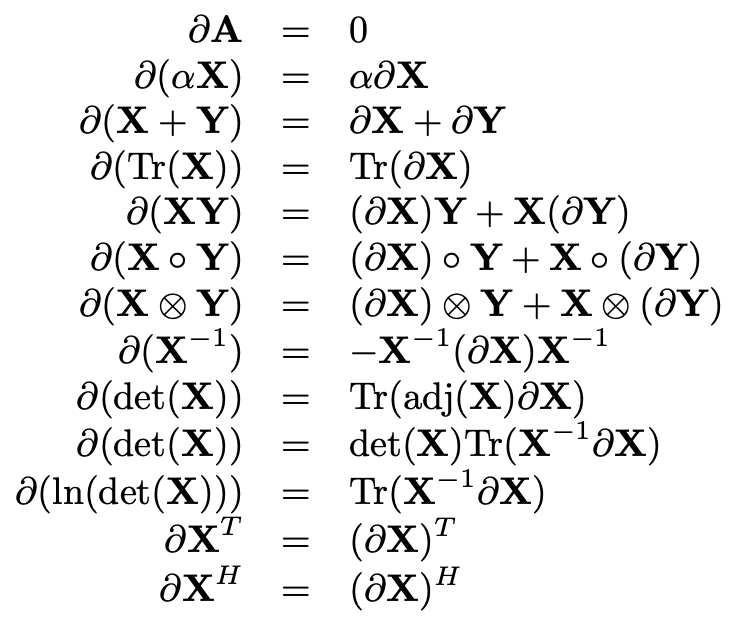
\includegraphics[width=.7\columnwidth]{src/matrix_deriv.png}

\subsection*{Matrices}

Cauchy-Schwarz: $\mathbf a^\top\mathbf b \leq \|\mathbf a\|_2\|\mathbf b\|_2$

Norms: $\mathbf w^\top\mathbf w=\|\mathbf w\|_2^2$, $\mathbf w^\top\text{sgn}(\mathbf w)=\sum_i |x_i|=\|\mathbf w \|_1$

Traces: $\text{Tr}(A+B)=\text{Tr}(A)+\text{Tr}(B)$, $\text{Tr}(AB)=\text{Tr}(BA)$, $\mathbf{a}^T \mathbf a = \text{Tr}(\mathbf{aa}^T)$, $\mathbf x^T\mathbf M\mathbf x=\text{Tr}(\mathbf x^T\mathbf M\mathbf x)$, $\mathbf x^T\mathbf y = \text{Tr}(\mathbf{yx}^T)$, if $\mathbf A$ s.p.d then $\text{Tr}(\mathbf A)\geq 0$.

Vector projection $\mathbf a$ to $\mathbf b$: $\frac{\mathbf a^\top \mathbf b}{\|\mathbf b\|^2}\mathbf b$

\iffalse
\subsection*{Parametric vs. Nonparametric}
\textbf{Parametric}: have finite set of parameters. 
e.g. linear regression, linear perceptron\\
\textbf{Nonparametric}: grow in complexity with the size of the data, more expressive.
e.g. k-NN
\fi
%\section*{Regression}
\textbf{SVD:}$\X=\mathbf{U}\Sigma\mathbf{V}^T$\\
\textbf{Model}:
$y=w_0 + \sum_{j=1}^d\mathbf{X_j} w_j$, $y\subset{\mathbb{R}}$\\
Introduce $X_0=1$ and rewrite\\
$y=\mathbf{X} \w \quad \mathbf{X}\in\mathbb{R}^{d\times n},  w \in \mathbb{R}^{d+1}$\\
Gau.noise$\epsilon \sim \mathcal{N}(0,\sigma^2)$;$y\sim \N(||\X||_2,\sigma^2)$\\
$\E[y|\X]=X^T w$
depending linearly on $(1,\x_1,...,\x_d)$;
$\hat{y}=\mathbf{X}\hat{ w}+\epsilon$\\
$\hat{ w} \sim \mathcal{N}( w, (\mathbf{X}^T\mathbf{X})^{-1}\sigma^2) $ and\\
$p(Y|X, w, \sigma) \sim \mathcal{N}(Y|X^T w, \sigma^2)$

% A Regression has Optimum:\\
% $f^*(x) = \mathbb{E}_Y[Y|X=x]$


\subsection*{Ordinary Least Squares}
$\hat R(w)=\sum_{i=1}^n(y_i-\w^T x_i)^2=||\y-\X\w||^2$\\
% $X\in\mathbb{R}^{n\times(d+1)}, y\in\mathbb{R}^n,   w\in\mathbb{R}^{d+1}$\\
$\hat \w = (\X^T\X)^{-1}\X^T\y=\mathbf{V}\Sigma^{-1}\mathbf{U}^T\y$\\
$\w^*$ \textbf{exists:} $\X^T\X$ invertible$\Leftrightarrow \X$full rank $\Leftrightarrow \X$ full column rank.
$\E_{\epsilon |\X}[\hat\w]=w\Rightarrow$ unbiased, $\V(\hat \w)=\sigma^2(\X^T\X)^{-1}$;
orth. projection with lowest variance of all unbiased estimates.\\
\textbf{Prediction:} $\hat{y}{=}\mathbf{X}\hat{ w}{=}\mathbf{X}(\mathbf{X}^T\mathbf{X})^{-1}\mathbf{X}^{T}\mathbf{y}$
\subsection*{Ridge Regression ($L^2$ penalty)}
$\hat R_{ridge}(w)=\sum_{i=1}^n(y_i-\w^T x_i)^2+\lambda\w^T\w=||\y-\X\w||^2+\lambda||\w||^2$;
$\hat \w_{ridge}(\lambda)=(\X^T\X+\lambda \I_d)^{-1}\X^T\y=\mathbf{V}(\Sigma^2+\lambda \I)^{-1}\Sigma\mathbf{U}^T\y$\\
$\E_{\epsilon |\X}[\hat\w_{r}]=(\X^T\X+\lambda\I)^{-1}(\X^T\X)\w$;biased
$\V(\hat \w_{ridge})=\sigma^2(\X^T\X+\lambda\I)^{-1}(\X^T\X)$\\$[(\X^T\X+\lambda\I)^{-1}]^T$;
$\V(\hat \w)\geq\V(\hat \w_{ridge})$;
%Bayes: $Y|(X, w)\sim\N(x^T w,\sigma^2\I)$;\\
%prior: $ w\sim\N(0,\frac{\sigma^2}{\lambda}\I)$;
$\hat R_{ridge}(w)$ convex $\Leftrightarrow$ Hessian $D^2\hat R_{ridge}(w)$ positive semi definite;
strictly convex; always unique sol; $\lambda \w^T\w$  biases sol. towards origin; shrinks the low variance components, $\Sigma_{jj}=d_{jj}\Rightarrow d_{jj}^{-1}\geq \frac{d_{jj}}{d_{jj}^2}+\lambda; \forall \lambda >0$

\subsection*{Lasso ($L^1$ penalty)}
$\hat R_{lasso}(\w) = ||\y-\X\w||^2+\lambda|| w||_1$\\
no closed form; sparse solutions $\rightarrow$ better generalization than ridge; convex;diamond

% \iffalse
% \subsection*{Bayesian Linear Regression}
% \textbf{Setting:} Define a prior over $ w$.\\
% \textbf{e.g. Ridge:} Assume $ w$ distributed as:\\
% $p( w|\bm{\bm{\Lambda}}){=}\mathcal{N}( w|\mathbf{0},\frac{\sigma^2}{\lambda}\mathbb{I}) \propto \mathrm{exp}(-\frac{\lambda}{2\sigma^2} w^T w)$\\
% For $\bm{\Lambda}=\frac{\sigma^2}{\lambda}\mathbb{I}$. Linear for $\sigma=1$.

% Then, given observed $\mathbf{X},\mathbf{y}$, use Bayes' theorem to find the posterior\\
% $p( w|\mathbf{X},\mathbf{y}, \bm{\Lambda}, \sigma) = \mathcal{N}(\mu_{ w}, \Sigma_{ w})$\\
% $\mu_ w = \sigma^2(\mathbf{X}^T\mathbf{X} +\sigma^2\bm{\Lambda})^{-1}\mathbf{X}^T\mathbf{y}$\\
% $\Sigma_ w = \sigma^2(\mathbf{X}^T\mathbf{X} +\sigma^2\bm{\Lambda})^{-1}$
% \fi

\subsection*{Nonlinear Regression}
basis expansion
\textbf{Idea:} Feature space transformation\\
Model: $\mathbf{Y}=f(\mathbf{X})=\sum_{i=1}^d\w_i \phi_i(\x)$\\
Transformation $\phi_i(\mathbf{X}):\mathbb{R}^d \rightarrow \mathbb{R}$

% \iffalse
% \section*{Bias-Variance tradeoff}
% Bias($\hat{f}$)$=\mathbb{E}[\hat{f}]-f$\\
% Var($\hat{f}$)$=\mathbb{E}[(\hat{f}-\mathbb{E}[\hat{f}])^2]$\\
% $|\mathcal{Z}|\downarrow \quad|\mathcal{F}|\uparrow\quad\Rightarrow\quad\mathrm{Var}\uparrow\quad\mathrm{Bias}\downarrow $\\
% $|\mathcal{Z}|\uparrow \quad|\mathcal{F}|\downarrow\quad\Rightarrow\quad\mathrm{Var}\downarrow\quad\mathrm{Bias}\uparrow $

% \subsection*{Squared Error Decomposition}
% $\mathbb{E}_D\mathbb{E}_{X,Y}[(\hat{f}(X)-Y)^2]=$\\
% $\mathbb{E}_{X,Y}[(\mathbb{E}_{Y|X}[Y]-Y)^2]$ (noise$^2$)\\
% $+\mathbb{E}_X\mathbb{E}_D[(\hat{f}_D(X)-\mathbb{E}_D[\hat{f}(X)])^2]$ (var.)\\
% $+\mathbb{E}_X[(\mathbb{E}_D[\hat{f}_D(X)]-\mathbb{E}_{Y|X}[Y])^2]$ (bias$^2$)\\
% With $\mathbb{E}_{Y|X}[Y]$ the expected label and $\mathbb{E}_{D}[\hat{f}(X)$ the expected classifier.
% \fi
%\section*{Model Selection}
\subsection*{K-Fold Cross Validation}
split training set:$K=\min\{\sqrt{n},10\}$\\
$\mathcal{Z}=\bigsqcup^{K}_{i=1}\mathcal{Z}_i $;
% with map $\kappa:\{1,\cdots, n\} \rightarrow\{, \cdots, K\}$
$|\mathcal{Z}_k|\approx n\frac{K-1}{K}$ \# of samples\\
%Learning:\\
$\hat{f}^{-\nu}(x){=}
\argmin_{f\in\mathcal{F}}\frac{\sum_{i\not\in\mathcal{Z}_\nu}(y_i-f(x_i))^2}{|\mathcal{Z}\setminus\mathcal{Z}_{\nu}|}$\\
%Validation:\\
$\hat{R}^{cv} = \frac{1}{n}\sum_{i\leq n}(y_i-\hat{f}^{-\kappa(i)}(x_i))^2$\\
Underfits because smaller dataset.\\
\textbf{Leave-one-out:} $K=n$ (unbiased but var can be large from corr. datasets)

% \subsection*{Bootstrapping}
% Bootstrap samples: $\mathcal{Z}^*=\{\mathcal{Z}_1^*, \cdots\mathcal{Z}_B^*\}$, of same size as original, drawn with replacement.
% The chance of a sample to have appeared in the bootstrap is:\\
% $1-(1-\frac{1}{n})\stackrel{n\to\infty}{\to} 1-\frac{1}{e}\approx 0.632$. So if we compute the ERM on $\mathcal{Z}$ we could get 63\% accuracy by memorization. Over-confident!\\
% \textbf{Leave-one-out}: compensates by computing the ERM where no memorization was for specific sample. E.g., for classification, like cross-validation:\\
% $\hat{\mathcal{R}}(S(\mathcal{Z}))=\frac{1}{B}\sum_{b=1}^B\sum_{z_i\not\in\mathcal{Z}^{*b}}\frac{\mathbb{I}_{c(x_i)\neq y_i}}{B-\lvert\mathcal{Z}^{*b}\rvert}$

% \subsection*{Jackknife}
% Estimate of an estimator $\hat{S}_n$'s Bias.\\
% $\hat{S}^{JK}=\hat{S}_n-\mathrm{bias}^{JK}$ is JK Estimator.\\
% $\mathrm{bias}^{JK}{=}(n{-}1)(\tilde{S}_n{-}\hat{S}_m)$\\
% $\tilde{S}_n{=}\frac{1}{n}\sum_{i=1}^n\hat{S}_{n{-}1}^{-i}$ avg. LOO Estimator.
% Debiased est. can have big variance!\\
% \textbf{Bootstrap debiased}\\ $\bar{S}{=}2\hat{S}{-}\frac{1}{B}\sum_b\hat{S}^*(b)$


%\section*{Classification}
% $w^* = \underset{w}{\operatorname{argmin}} ~ l(w;x_i,y_i)$
\subsection*{Metrics $n = n_+ + n_- = p_+ + p_-$}
$n_+ = \text{TP} + \text{FN}$, $n_- = \text{TN} + \text{FP}$, $p_+ = \text{TP} + \text{FP}$, $p_- = \text{FN} + \text{TN}$
Accuracy: $\frac{\text{TP}+\text{TN}}{n}$; \\
Precision: $\frac{\text{TP}}{\text{TP}+\text{FP}}$
Recall/TPR: $\frac{\text{TP}}{n_+}$; \\
FPR: $ \frac{\text{FP}}{n_-}$;
F1:$\frac{2TP}{2TP+FP+FN}=\frac{2}{\frac{1}{\text{Precision}}+\frac{1}{\text{Recall}}}$\\
ROC Curve: $y = $TPR, $x = $FPR; $A1 \succ A2$ in ROC $\Leftrightarrow A1 \succ A2$ in precision/recall curve
% $F_1=2\frac{\text{pre}*\text{rec}}{\text{pre}+\text{rec}}$\\
\subsection*{Loss}
$l_{0/1}(\w;\x_i,y_i)=1:\; \text{if}\;y_i\neq \text{sign}(\w^T\x_i), 0:\text{else}$\\
$l_{P}(\w;\x_i,y_i)=\max(0,-y_i\w^Tx_i)$, conv.surrogate for $l_{0/1}$;\\
$l_{H}(\w;\x_i,y_i)=\max(0,1-y_i\w^T\x_i)$
\subsection*{Perceptron}
SGD on $l_P$ with $\eta=1$;
$\nabla_w l_P(w;y_i,x_i) = 
\begin{cases}
    0 &\text{if } y_i w^T x_i \geq 0\\
    -y_i x_i &\text{otherwise}
\end{cases}$ \\
% \subsection*{Linear Classifier}
% % optimal for Gaussian with equal cov. Stat. simplicity \& comput. efficiency.
% $g(x)=a^T\tilde{x}\quad a=(w_0,w)^T, \tilde{x}=(1,x)^T$\\
% $a^T\tilde{x}_i>0 \Rightarrow y_i=1, a^T\tilde{x}_i<0 \Rightarrow y_i=2$\\
% Normalization: $\tilde{x}_i\rightarrow-\tilde{x}_i$ if $y_i=2$
% Find $a$: $a^T\tilde{x}_i>0,\forall i$

% \subsection*{Perceptron Criterion}
% $J_P(a)=\sum_{\tilde{x}\in\mathcal{X}^\text{msc}}(-a^T\tilde{x})$,\\
% $\mathcal{X}^\text{msc}$: set of misclassified samples.\\
% $\Rightarrow a(k+1)=a(k)+\eta(k) \sum_{\tilde{x}\in\mathcal{X}^\text{msc}} \tilde{x}$\\
% Converges if data separable.\\
% Single sample perceptron: $(k++)\mod n$\\
% $a(k+1)=a(k)+\tilde{x}^k$ (misclassified).

%\subsection*{Fisher's Linear Discriminant Analysis}
%Maximize distance of the means of the projected classes to find projection plane separating them best.\\
%proj mean: $\tilde{m}_{\alpha}{=}\frac{1}{n_{\alpha}}\sum_{x\in\mathcal{X}_{\alpha}}w^Tx{=}w^Tm_{\alpha}$\\
%Dist of proj means: $|w^T(m_1-m_2)|$
%Classes proj. cov: $\tilde{\Sigma}_1{+}\tilde{\Sigma}_2{=}w^T(\Sigma_1{+}\Sigma_2)w$\\
%Fishers Criterion:\\
%$J(w)=\frac{||m_1-m_2||^2}{\tilde{\Sigma}_1{+}\tilde{\Sigma}_2}=\frac{w^T(m_1-m_2)(m_1-m_2)^Tw}{w^T(\Sigma_1{+}\Sigma_2)w}$
%Fishers Crit for Multiple Classes:\\
%$J(W)=\frac{|W^T\Sigma_BW|}{W^T\Sigma_WW}$\\
%$\Sigma_B=\sum_{i=1}^kn_k(m_k-m)(m_k-m)^T$\\
%$\Sigma_W=\sum_{i=1}^k\sum_{x\in \mathcal{D}_i}(x-m_i)(x-m_i)^T$

% \textbf{LDA for Multiclasses}: 
% Reformulate as $(k-1)$ ``class $\alpha$ - not class $\alpha$'' dichotomies. But some area are ambiguous

\subsection*{Support Vector Machine (SVM)}
$\nabla_w l_H(w;y,x) = 
\begin{cases}
    0 &\text{if } y_i w^T x_i \geq 1\\
    -y_i x_i &\text{otherwise}
\end{cases}$\\
$w^* = \argmin_\w ~\frac{1}{n}\sum_{i=1}^nl_H(w;x_i,y_i)+\lambda||w||_2^2$\\ For L1-SVM (feature selection) use $||w||_1$ 
save learning rate: $\eta_t=\frac{1}{\lambda t}$
% Generalize Perceptron with margin $m$ and kernel. Find plane that $\max  m$ s.t.:\\
% $z_ig(\mathbf{y})=z_i(\mathbf{w}^T\mathbf{y}+w_0)\geq m,\forall \mathbf{y}_i \in \mathcal{Y}$\\
% $z_i \in \{-1,+1\}\quad \mathbf{y_i} = \phi(\mathbf{x_i})$\\
% \textbf{Support Vectors:} $\mathbf{y}_i$ with $z_ig(\mathbf{y}_i)=m$
% Functional Margin Problem:\\
% minimizes $||\mathbf{w}||$ for $m{=}1$: 
% $L(\mathbf{w}, w_0, \mathbf{\alpha}) {=}$\\
% $=\frac{1}{2}\mathbf{w}^T\mathbf{w}{-}\sum_{i=1}^n\alpha_i[z_i(\mathbf{w}^T\mathbf{y}_i{}+w_0){-}1]$\\
% where $\alpha_i$ are Lagrange multipliers.
% $\frac{\partial L}{\partial w} {=} 0$\\ $\frac{\partial L}{\partial w_0} {=} 0 \Rightarrow \mathbf{w}=\sum_{i=1}^n\alpha_iz_i\mathbf{y_i} \quad 0=\sum_{i=1}^n\alpha_iz_i$\\
% %Replacing these in $L(\mathbf{w}, w_0, \mathbf{\alpha})$ we get\\
% $\tilde{L}(\mathbf{\alpha}){=}\sum_{i=1}^n\alpha_i{-}\frac{1}{2}\sum_{i,j=1}^n\alpha_i\alpha_jz_iz_j\mathbf{y_i}^T\mathbf{y_j}$
% max
% with$\alpha_i\geq0\quad$  $\quad\sum_{i=1}^n\alpha_iz_i=0$; Dual\\
% optimal hyperplane:
% $\mathbf{w^*}=\sum_{i=1}^n\alpha_i^*z_i\mathbf{y_i}$\\
% $ w_0^*{=}{-}\frac{1}{2}(\mathrm{min}_{z_i=1}\mathbf{w^*}^T\mathbf{y_i}{+}\mathrm{max}_{z_i=-1}\mathbf{w^*}^T\mathbf{y_i})$\\
% Only Support Vectors ($\alpha_i\not=0$) contribute to the evaluation.\\
% Optimal Margin: $\mathbf{w}^T\mathbf{w}=\sum_{i\in SV}\alpha_i^*$\\
% Discrim.: $g^*(\mathbf{y}){=}\sum_{i\in SV}z_i\alpha_i\mathbf{y_i}^T\mathbf{y}{+}w^*_0$\\
% $\mathrm{class} = \mathrm{sign(\mathbf{y}^T\mathbf{w}^*+w_0^*)}$

% \subsection*{Soft Margin SVM}
% Introduce slack to relax constraints\\
% $z_i(\mathbf{w}^T\mathbf{y}_i+w_0)\geq m(1-\xi_i)$; $\xi_i \geq 0$\\
% $L(\mathbf{w}, w_0,\mathbf{\xi}, \mathbf{\alpha}, \mathbf{\beta}) {=}\frac{1}{2}\mathbf{w}^T\mathbf{w}+C\sum_{i=1}^n\xi_i-$\\
% ${-}\sum_{i=1}^n\alpha_i[z_i(\mathbf{w}^T\mathbf{y}_i{+}w_0){-}1{+}\xi_i]$\\
% ${-}\sum_{i=1}^n\beta_i\xi_i$; $\, \frac{\partial L}{\partial\xi_i}= C-\alpha_i-\beta_i=0$\\
% $C\downarrow\Rightarrow m\downarrow\wedge\mathrm{constrain}\, \mathrm{violation}\downarrow$ \\
% Dual constraints:
% $C \geq \alpha_i \geq 0$

% \subsection*{Non-Linear SVM}
% Use kernel in discriminant funct: $g(\mathbf{x})=\sum_{i,j=1}^n\alpha_i\alpha_jz_iz_jK(\mathbf{x_i},\mathbf{x})$\\
% E.g solve the XOR Problem with:
% $K(x,y)=(1+x_1y_1+x_2y_2)^2$

% \subsection*{Multiclass SVM}
% $\forall$class $z\in\{1,2,\cdots,M\}$ introduce $\mathbf{w}_z$ and define the margin $m$ s.t.:  $\min_{\mathbf{w_z}}\frac{1}{2}\sum_{z=1}^M\mathbf{w}_z^T\mathbf{w}_z$\\
% $(\mathbf{w}_{z_i}^T\mathbf{y}_i+w_{z_i,0})-\max_{z\not=Z_i}(\mathbf{w}_z^T\mathbf{y}_i+w_{z,0})\geq m, \forall{\mathbf{y}_i\in \mathcal{Y}}$

% \subsection*{Structured SVM}
% Each sample $\mathbf{y}$ is assigned to a structured output label $z$\\
% Output Space Representation:\\
% joint feature map: $\mathbf{\psi}(z,\mathbf{y})$\\
% Scoring function: $f_{\mathbf{w}}(z,\mathbf{y})=\mathbf{w}^T\mathbf{\psi(z, \mathbf{y})}$\\
% Classify: $\hat{z}=h(\mathbf{y})\argmax_{z\in\mathcal{K}}f_{\mathbf{w}(z, \mathbf{y})}$
\subsection*{Multi class}
$l_{MC-H}(w^{(1)},...,w^{(c)};x,y) =
\max (0,1+\max_{j\in\{1,\cdots,y-1,y+1,\cdots,c\}} w^{(j)T} x - w^{(y)T} x)$
%\section*{Feature selection}
\subsection*{Greedy feature selection}
slow, high computational cost;
applies to any prediction method
\subsubsection*{Forward}
start with 0 feat. add best feat as long as error decreases.
\textbf{Problem:} 1 feature $\Rightarrow$ 50\% error rate;
usually faster
\subsubsection*{Backward}
start with all feat. remove worst feat as long as error decreases.
Can handle dependent feat.
\subsection*{L1 as surrogate for L0}
fast,(training and feat selection happen jointly);
only works for linear models
%\section*{Kernels $K(\mathbf{x}, \mathbf{x'}) {=} \phi(\mathbf{x})^T\phi(\mathbf{x'})$}
Similarity based reasoning\\
Gram Matrix $K{=}K(\mathbf{x}_i, \mathbf{x}_j), 1{\leq} i,j{\leq} n$\\
sym. p.s.d.(all EV $\geq$ 0); Engineering:\\
$K_1(\mathbf{x}, \mathbf{x'})K_2(\mathbf{x}, \mathbf{x'})$; 
$\alpha K_1(\mathbf{x}, \mathbf{x'})+\beta K_2(\mathbf{x}, \mathbf{x'})$\\
$\phi:\mathcal{X}{\rightarrow}\mathcal{X},\,\,K(\phi(\mathbf{x}), \phi(\mathbf{x'}))$; $p(h|\mathbf{x})p(h'|\mathbf{x'})$\\ 
$h: \mathrm{poly/exp},\,\, h(K(\mathbf{x}, \mathbf{x'}))$;$ \, f(\mathbf{x})K(\mathbf{x},\mathbf{x'})f(\mathbf{x'})$

lin/poly: $\mathbf{x}^T\mathbf{x'}$; $(\mathbf{x}^T\mathbf{x'}{+}1)^p$;
$\mathrm{dim}=\binom{n+p}{p}$\\
RBF(Gauss): $\exp(-||\mathbf{x}{-}\mathbf{x'}||_2^2/h^2)$\\
lapl: $\exp(-||\mathbf{x}{-}\mathbf{x'}||_1/h)$, $h\uparrow$: regularizat.\\
Sigmoid:$\mathrm{tanh}(\alpha\mathbf{x}^T\mathbf{x'}+c)$\\
not p.s-d eg: $\mathbf{x}{=}[1,-1], \mathbf{x'}{=}[-1,2]$

\subsection*{Reformulating the perceptron}
Ansatz: $w^* \in \operatorname{span}(X) \Rightarrow w = \sum_{j=1}^n \alpha_j y_j x_j$\\
$\alpha^*= \argmin_{\alpha} \frac{1}{n} \sum_{i=1}^n \max(0,$\\$- \sum_{j=1}^n \alpha_j y_i y_j x_i^T x_j)$

\subsection*{Kernelized perceptron and SVM}
Use $\alpha^T k_i$ instead of $w^T x_i$,\\
use $\alpha^T D_y K D_y \alpha$ instead of $||w||_2^2$\\ 
$k_i=[y_1 k(x_i,x_1), ..., y_n k(x_i,x_n)]$;\\
$D_y = \text{diag}(y)$\\
Prediction: $f(\hat{x}) = \operatorname{sign}(\sum_{i=1}^n \alpha_i y_i k(x_i, \hat{x}))$

\subsection*{Kernelized linear regression (KLR)}
Ansatz: $w^*=\sum_{i = 1}^n \alpha_i x$\\
$\alpha^*= \argmin_{\alpha}\frac{1}{n} ||\alpha^T K - y||_2^2 + \lambda \alpha^T K \alpha \\= (K+\lambda I)^{-1} y$\\
Prediction: $f(\hat{x}) = \sum \limits_{i=1}^n \alpha_i k(x_i,\hat{x})$

% TODO commented this out because there were errors
%\section*{Neural network}
Parameterize feature map: $\phi(x,\theta)$ instead of $\phi(x)$, usually: $\phi(x,\theta) = \varphi(\theta^T x) = \varphi(z)$\\
$\Rightarrow w^* = \underset{w, \theta}{\operatorname{argmin}} \sum_{i=1}^n l(y_i; \sum_{j=1}^m w_j \phi(x_i, \theta_j))$

\subsection*{Activation functions}
Sigmoid: $\sigma(z)=\frac{1}{1+e^{-z}}$,\\
$\sigma'(z) = (1 - \sigma(z))\cdot\sigma(z)$\\
Tanh: $\varphi(z) = tanh(z) = \frac{exp(z)-exp(-z)}{exp(z)+exp(-z)}$\\
ReLu:  $\varphi(z) = max(z,0)$

\subsection*{Predict: forward propagation}
$v^{(0)} = x$; for $l = 1,...,L-1$:
$v^{(l)} = \varphi(z^{(l)})$; $z^{(l)} = W^{(l)}v^{(l-1)}$;
$f = W^{(L)}v^{(L-1)}$\\
Predict $f$ for regression, $\operatorname{sign}(f)$ for class.

\subsection*{Compute gradient: backpropagation}
Output layer: 
$\delta_j = l_j'(f_j)$,
$\frac{\partial}{\partial w_{j,i}} = \delta_j v_i$\\
Hidden layer $l=L-1,...,1$:\\
$\delta_j = \varphi'(z_j) \cdot \sum_{i\in Layer_{l+1}} w_{i,j}\delta_i$,
$\frac{\partial}{\partial w_{j,i}} = \delta_j v_i$

\subsection*{Learning with momentum}
$a \leftarrow m \cdot a + \eta_t \nabla_W l(W;y,x)$; $W \leftarrow W - a$
%\section*{Clustering}
\subsection*{k-mean}

$\hat{R}(\mu) = \sum_{i=1}^n \underset{j\in\{1,...k\}}{\operatorname{min}}||x_i-\mu_j||_2^2$\\
$\hat{\mu} =  \argmin_{\mu} ~ \hat{R}(\mu)$;non-convex, NP-hard \\
\subsubsection*{Algorithm (Lloyd's heuristic)}
Init: $\mu^{(0)}$; while not converged:\\
$z_i^{(t)}=\argmin_{j \in \{1,...,k\}}||\x_i-\mu_j^{(t-1)}||_2^2$;
$\mu_j^{(t)}=\frac{1}{|\{i:z_i^{(t)}=j\}|}\sum_{i:z_i^{(t)}=j}x_i$; $O(nkd)$per iter
% Choose starting centers, assign points to closest center, update centers to mean of each cluster, repeat

%\subsection*{k-mean++}
%- Start with random data point as center\\
%- Add centers 2 to k randomly, proportionally to squared distance to closest selected center\\
%for $j=2$ to $k$:
%$i_j$ sampled with prob.\\
%$P(i_j=i) = \frac{1}{z} \underset{1\leq l<j}{min}||x_i-\mu_l||_2^2$; $\mu_j \leftarrow x_{i_j}$
%\section*{Dimension reduction}
\subsection*{PCA}
$D\subset \mathbb{R}^d$; $\mu = \frac{1}{n}\sum_{i=1}^nx_i=0$; 
$\Sigma = \frac{1}{n}\sum_{i=1}^n x_i x_i^T$\\
$(W,z_1,...,z_n) = \operatorname{argmin} \sum_{i=1}^n||W z_i - x_i||_2^2$;\\
$W = (v_1|...|v_k) \in \mathbb{R}^{d \times k}$ ortho; $z_i = W^T x_i$ \\ 
$v_i$ eigenvec of $\Sigma$

\subsection*{Kernel PCA}
$\alpha^{(1)},...,\alpha^{(k)}\in \mathbb{R}^n$, $\alpha^{(i)} = \frac{1}{\sqrt{\lambda_i}}v_i$, $K = \sum_{i=1}^n \lambda_i v_i v_i^T$, $\lambda_1 \geq ... \geq \lambda_d \geq 0$\\
New p: $z = f(\x) = \sum_{j=1}^n\alpha_j^{(i)}k(\x,x_j)$; $z\in \R^k$

\subsection*{Autoencoders}
Find identity function: $x \approx f(x;\theta)$\\
$f(x;\theta) = f_{decode}(f_{encode}(x;\theta_{encode});\theta_{decode})$
%\section*{Probability modeling}
Find $h:X\rightarrow Y$ that min. pred. error: 
$R(h) = \int P(x,y)l(y;h(x)) \partial yx \partial y = \mathbb{E}_{x,y}[l(y;h(x))]$

\subsection*{For least squares regression}
Best $h$: $h^*(x) = \mathbb{E}[Y|X=x]$ \\
Pred.: $\hat{y} = \hat{\mathbb{E}}[Y|X=\hat{x}] = \int \hat{P}(y|X=\hat{x}) y \partial y$

\subsection*{MLE}
$\theta^* = \underset{\theta}{\operatorname{argmax}} ~ \hat{P}(y_1,...,y_n|x_1,...,x_n,\theta)$\\
lin. + Gauss: $y_i = w^T x_i + \varepsilon_i, \varepsilon_i \sim \mathcal{N}(0, \sigma^2)$\\
i.e. $y_i \sim \mathcal{N}(w^T x_i, \sigma^2)$, With MLE (use\\ $\operatorname{argmin} ~ - \operatorname{log}$): $w^* = \underset{w}{\operatorname{argmin}} \sum (y_i-w^Tx_i)^2$

\subsection*{Bias/Variance/Noise}
Pred error = $Bias^2 + Variance + Noise$

\subsection*{MAP}
Assume bias on parameters, e.g. $w_i \in \mathcal{N}(0, \beta^2)$;
Bay.: $P(w|x,y) = \frac{P(w|x) P(y|x,w)}{P(y|x)} = \frac{P(w) P(y|x,w)}{P(y|x)}$
\subsection*{Logistic regression}
sigmoid:$\sigma(w^Tx) = \frac{1}{1+exp(-w^Tx)}$\\
$P(y|x,w) = Ber(y; \sigma(w^Tx)) = \frac{1}{1+exp(-y w^T x)}$\\
\textbf{CLF}: Use $P(y|x,w)$, predict most likely class label.
\subsubsection*{MLE}
$\underset{w}{\operatorname{argmax}} ~ P(y_{1:n}|w,x_{1:n})\\
w^* = \underset{w}{\operatorname{argmin}} \sum_{i=1}^n log(1+exp(-y_i w^T x_i))$\\
\textbf{SGD}: $w = w + \eta_t y x \hat{P}(Y = -y|w,x)$\\
$\hat{P}(Y = -y|w,x) = \frac{1}{1+exp(yw^Tx)}$
\subsubsection*{MAP} Gauss. prior: $||w||_2^2$, Lap. prior: $||w||_1$\\
\textbf{SGD}: $w = w (1-2\lambda \eta_t) + \eta_t y x \hat{P}(Y = -y|w,x)$
%\section*{Bayesian decision theory}
- Cond. dist. over labels $P(y|x)$\\
- Set of actions $\mathcal{A}$\\
- Cost function $C:Y\times \mathcal{A} \rightarrow \mathbb{R}$\\
$a^* = \underset{a \in \mathcal{A}}{\operatorname{argmin}} ~ \mathbb{E}[C(y,a)|x]$\\
\subsubsection*{Classification} $C(y,a) = [y \not = a]$; asymmetric: \\
$C(y,a) =
 \begin{cases}
 	c_{FP} \text{ , if $y=-1$, $a=+1$}\\
		c_{FN} \text{ , if $y=+1$, $a=-1$}\\
		0 \text{ , otherwise}
 \end{cases}$
\subsubsection*{Regression}  $C(y,a) = (y-a)^2$; asymmetric: $C(y,a) = c_1 \max(y-a,0) + c_2 \max(a-y,0)$
% E.g. $y \in \{-1,+1\}$, pred$+$if $c_+ < c_-$,\\
% $c_+ = \mathbb{E}(C(y, +1)|x) = P(y = 1|x) \cdot 0 + P(y = -1|x) \cdot c_{FP}$, $c_-$ likewise

%\subsection*{Optimal decision for logistic regression}
%$a^* = \underset{y}{argmax} \hat{P}(y|x) = sign(w^T x)$

% \subsection*{Example: logistic regression}
% \begin{itemize}
% 	 Est. cond. dist: $P(y|x,w) = Ber(\sigma(w^Tx))$
% 	 Action set: $\mathcal{A} = \{ +1, -1\}$
% 	 Cost function: $C(y,a) = [y \not = a]$ \\ 
% 	$= \left \{ 
% 		\begin{array}{lr}
% 			1 \text{ , if } y \not = a\\
% 			0 \text{ , otherwise}
% 		\end{array}
% 		$
% \end{itemize}
% $a^* = \underset{a \in \mathcal{A}}{\operatorname{argmin}} \mathbb{E}_y[C(y,a)|x]$\\
% $= \underset{a \in \mathcal{A}}{\operatorname{argmin}} P(y=1|x,w)[a=1] + P(Y=-1|x,w)[a=+1]$\\
% $= \underset{a \in \mathcal{A}}{\operatorname{argmin}} P(y \not = a | x,w) = \underset{a \in \mathcal{A}}{\operatorname{argmin}} \frac{1}{1+exp(aw^Tx)}$\\
% $=\underset{a \in \mathcal{A}}{\operatorname{argmax}} (1 + exp(aw^Tx))$
% $=\underset{a \in \mathcal{A}}{\operatorname{argmax}} (aw^Tx)$\\
% $= sign (w^Tx)$

%\subsection*{Example: Asymmetric costs}
%	 Est. cond. dist: $\hat{P}(y|x,w) = Ber(\sigma(w^Tx))$
%	 Action set: $\mathcal{A} = \{ +1, -1\}$
%	 Cost function: $C(y,a) =
%	 \begin{cases}
%	 	c_{FP} \text{ , if $y=-1$ and $y=+1$}\\
%			c_{FN} \text{ , if $y=+1$ and $y=-1$}\\
%			0 \text{ , otherwise}
%	 \end{cases}
%		$
%The action that minimizes the expected cost is:\\
%$C_+ = \mathbb{E}_y[C(y,+1)|x] = P(y=+1|x) \cdot 0 + (P(y=-1)|x) \cdot c_{FP}$\\
%$C_- = \mathbb{E}_y[C(y,-1)|x] = P(y=+1|x) \cdot c_{FN} + P(y=-1|x) \cdot 0$\\
%Predict +1 if $C_+ \leq C_- \Leftrightarrow P(y=+1|x) \geq \frac{c_{FP}}{c_{FP} + c_{FN}}$

%\subsection*{Doubtful logistic regression}
%	 Est. cond. distr.: $\hat{P}(y|x) = Ber(y;\sigma(\hat{w}^Tx))$\\
%	 Action set: $\mathcal{A} = \{ +1, -1, D\}$;  Cost function:\\
%	 $C(y,a) = \begin{cases}
%			[y \neq a] &\text{if } a \in \{+1,-1\}\\
%			c &\text{if } a = D
%       \end{cases}$\\
%The action that minimizes the expected cost\\
%$a^* = y \text{ if } \hat{P}(y|x) \geq 1-c\text{, D otherwise}$
%$a^* = \begin{cases}
%		y &\hat{P}(y|x) \geq 1-c\\
%		D &\text{otherwise}
%	   \end{cases}
%$

%\subsection*{Least squares regression}
%	 Est. cond. distr.: $\hat{P}(y|x,w) = \mathcal{N}(y;w^Tx, \sigma^2)$\\
% $\mathcal{A} = \mathbb{R}$; $C(y,a) = (y-a)^2$\\
%The action that minimizes the expected cost\\
%$a^* = \mathbb{E}_y[y|x] = \int \hat{P}(y | x) \partial y = \hat{w}^Tx$

%\subsection*{Asymmetric cost for regression}
%	 Est. cond. distr.: $\hat{P}(y|x) = \mathcal{N}(\hat{y};\hat{w}^Tx, \sigma^2)$\\
%	 $\mathcal{A} = \mathbb{R}$; $C(y,a) = c_1 \max(y-a,0) + c_2 \max(a-y,0)$
%Action that minimizes the expected cost:\\
%$a^* = \hat{w}^Tx + \sigma \Phi^{-1} (\frac{c_1}{c_1 + c_2})$, $\Phi$: Gaussian CDF\\
%$\frac{\partial}{\partial a}$\\
%$\frac{\partial}{\partial a} \mathbb{E}_y[C(y,a)|x] = \int_{-\infty}^{\infty} C(y,a) P(y | x) dy \overset{!}{=} 0$\\
%$= -c_1 \int_{a}^{\infty} P(y | x) dy + c_2 \int_{-\infty}^{a} P(y | x) dy$\\
%$= -c_1 [1-\phi(a; w^Tx, \sigma^2)] + c_2 \phi(a; w^Tx, \sigma^2)$\\
%$\phi(a; w^Tx, \sigma^2) = \frac{c_1}{c_1 + c_2}$\\
%using $\phi(u;v,w) = \phi((u-v)/\sqrt{w};0,1)$ and applying inverse CDF of std. ND $\phi^{-1}$ we get\\
%$a^* = w^Tx + \sigma\phi^{-1} (\frac{c_1}{c_1 + c_2})$
%\section*{Generative modeling}
estimate joint: $P(y,\x)$; can derive cond from joint;
1. generate class labels: $P{(y)}$ \textbf{MLE};
2. generate feat given class: $P(\x|y)$ \textbf{MLE};
3. obtain pred: $P(y|\x)=\frac{P(y)P(\x|y)}{Z}$,
$Z=P(\x)=\sum_yP(\x,y)=\sum_yP(y)P(\x|y)$ \textbf{MAP};
\subsection*{Discriminative}
estimate cond: $P(y|\x)$; not modeling $P(\x)$;
no outlier detection

\subsection*{Naive Bayes}
$P(Y=y)=p_y$; $y\in\mathcal{Y}=\{1,...,c\}$;$\sum_yp_y=1$
cond ind:
$P(X_1,...,X_d|Y)=\prod_{i=1}^dP(X_i|Y)$\\
$P(\X=(x_1,...,x_d))=\sum_yp((x_1,...,x_d),y)=\sum_yp((x_1,...,x_d)|y)p_y$


\subsection*{Examples}
\subsubsection*{multivar. Bernouilli Naive Bayes}
$p(\x_i|y=c)=\prod_{j=1}^d\text{Ber}(x_{ij}|\mu_{jc})$\\
% \subsubsection*{categorical Naive Bayes}
% $p(x|y=c,\theta)=\prod_{i=1}^d\prod_{}$\\
MLE for $P(Y=y) = p_y = \frac{\text{Count}(Y=y)}{n}$\\
% MLE for $P(x_i|y) = \mathcal{N}(x_i;\mu_{i,y}, \sigma_{i,y}^2)$:\\
% $\hat{\mu}_{i,y} = \frac{1}{\text{Count}(Y=y)} \sum_{x\in D_{x_i|y}} x$\\
% $\hat{\sigma}_{i,y}^2 = \frac{1}{\text{Count}(Y=y)} \sum_{x\in D_{x_i|y}} (x-\hat{\mu}_{i,y})^2$\\
MLE for Poi.: $\lambda = \operatorname{avg}(x_i) $\\
$\mathbb{R}^d$: $P(X = x|Y = y) = \prod_{i=1}^dPois(\lambda_y^{(i)},x^{(i)})$


\subsection*{Deriving decision rule}
%In order to predict label y for new point x, use\\
$P(y|x) = \frac{1}{Z} P(y)P(x|y)$, $Z = \sum_y P(y) P(x|y)$\\
$y^* = \argmax_y P(y|x) = 
\argmax_y P(y) \prod_{i=1}^d P(x_i|y)$;
$P_1-P_0\geq0$

\subsection*{Gaussian Bayes Classifier}
$\hat{P}(x|y) = \mathcal{N}(x ; \hat{\mu}_y, \hat{\Sigma}_y)$\\
$\hat{P}(Y=y) = \hat{p}_y = \frac{n_y}{n}$\\
$\hat{\mu}_{y} = \frac{1}{n_y} \sum_{i:y_i=y} x_i \in \mathbb{R}^d$\\
$\hat{\Sigma}_{y} = \frac{1}{n_y} \sum_{i:y_i=y} (x_i - \hat{\mu}_{y})(x_i-\hat{\mu}_y)^T \in \mathbb{R}^{d \times d}$

\subsection*{Fisher's lin. discrim. analysis (LDA, c=2)}
Assume: $p = 0.5$; $\hat{\Sigma}_- = \hat{\Sigma}_+ = \hat{\Sigma}$\\
discriminant function: 
$f(x) = \operatorname{log} \frac{p}{1-p} + \\
\frac{1}{2}[\operatorname{log} \frac{|\hat{\Sigma}_-|}{|\hat{\Sigma}_+|}
+ \left((x - \hat{\mu}_-)^T \hat{\Sigma}_-^{-1} (x - \hat{\mu}_-)\right) - \\
\left((x - \hat{\mu}_+)^T \hat{\Sigma}_+^{-1} (x - \hat{\mu}_+)\right)]$\\
Predict: $y = \operatorname{sign}(f(x)) = \operatorname{sign} (w^T x + w_0)$\\
$w = \hat{\Sigma}^{-1}(\hat{\mu}_+ - \hat{\mu}_-)$; \\
$w_0 = \frac{1}{2}(\hat{\mu}_-^T\hat{\Sigma}^{-1}\hat{\mu}_- - \hat{\mu}_+^T \hat{\Sigma}^{-1}\hat{\mu}_+)$

\subsection*{Outlier Detection}
$P(x) \leq \tau$

\subsection*{Categorical Naive Bayes Classifier}
MLE for feature distr.:\\
$\hat{P}(X_i = c|Y = y) = \theta_{c|y}^{(i)}\\
\theta_{c|y}^{(i)} = \frac{Count(X_i = c, Y = y)}{Count(Y=y)}$\\
Prediction: $y^* = \underset{y}{argmax}\hat{P}(y|x)$

% TODO commented this out because there were errors
%\section*{Missing data}
\subsection*{Mixture modeling}

Model each c. as probability distr. $P(x|\theta_k)$\\
$P(D|\theta) = \prod_{n=1}^N \sum_{k=1}^K \pi_k P(x_n|\theta_k)$\\
$L(\theta) = - \sum_{n=1}^N \operatorname{log}  \sum_{k=1}^K \pi_k p_k(x_n| \theta_k)$

\subsection*{Hard-EM algorithm}
Init: $\theta^{(0)}=(\pi_1,...,\pi_K, \theta_1,...,\theta_K)$ rand.
\textbf{E-step}: Predict most likely class for each point:
$z_i^{(t)} = \underset{z}{\operatorname{argmax}} ~ P(z|x_i, \theta^{(t-1)})\\
= \underset{z}{\operatorname{argmax}} ~ P(z|\theta^{(t-1)}) P(x_i|z,\theta^{(t-1)})$;\\
\textbf{M-step}: Compute the MLE: $\theta^{(t)} = \underset{\theta}{\operatorname{argmax}} P(D^{(t)}|\theta)$, i.e. $\mu_j^{(t)} = \frac{1}{n_j} \sum_{i: z_i = j x_j}$

\subsection*{Soft-EM algorithm}
\subsubsection*{E-step} Calc prob for each data point and class:
$r_{nk}=\E_Q[Z_n]=\gamma_k(x_n)=p(z_n=k|\x_n)=\frac{\pi_kp_k(\x_n|\theta_k)}{\sum_{k=1}^K\pi_kp_k(\x_n|\theta_k)}$;
$z_n=\argmax_k \gamma_k(x_n)$
\subsubsection*{M-step} Fit clusters to weighted data points:
$L(\theta)=\E_Q[p(x,z|\theta)]=\sum_{n=1}^N\sum_{k=1}^Kr_{nk}(\log(\pi_kp_k(\x_n|\theta_k)))$
$\pi_k = \frac{\sum_{n=1}^N \gamma_k (\x_n)}{N} $; 
$\mu_k = \frac{\sum_{n=1}^N \gamma_k (\x_n) \x_n}{\sum_{n=1}^N \gamma_k (\x_n)}\\ %\text{|learning with GMMs } ^t = ^*\\
\sigma_k = \frac{\sum_{n=1}^N \gamma_k(\x_n) (\x_n - \mu_k)^T (\x_n - \mu_k)}{\sum_{n=1}^N \gamma_k(\x_n)}$

 \subsection*{Soft-EM for semi-supervised learning}
labeled $y_i$: $\gamma_j^{(t)}(x_i) = [j = y_i]$,
unlabeled:\\ $\gamma_j^{(t)}(x_i) = P(Z=j|x_i, \mu^{(t-1)}, \Sigma^{(t-1)}, w^{(t-1)})$
\subsection*{Gaussian-Mixture Bayes classifiers}
Estimate prior $P(y)$; Est. cond. distr. for each class:
$P(x|y) = \sum_{j=1}^{k_y} w_j^{(y)} \mathcal{N}(x; \mu_j^{(y)}, \Sigma_j^{(y)})$\\
\subsection*{Examples}
\subsubsection*{k binary variables $X_1,..,X_K$}
$P(X_i=1|Y=y)=\theta_{i|y}$;$P(Y=y)=\theta_y$
$p(\x_i,y_i;\theta)=\theta_{y_i}\prod_{k=1}^K\theta_{k|y_i}^{x_{i,k}}(1-\theta_{k|y_i})^{1-x_{i,k}}$

\subsubsection*{1D Laplacian}
$\argmax_{\mu_k}-\sum_{n=1}^N\frac{\gamma_k(x_n)}{\beta_k}|x_n-\mu_k|$; 1D-conv opt problem, function p.w. linear,
breaking points: $D=x_1,x_2,...,x_n$$\Rightarrow$ optimum$\in D \Rightarrow \mu_k=x_n$ with largest obj. value.
% \subsection*{Log-likelihood}
% $l(\theta) = log P(\mathcal{D})$ \\
% $=\sum_{\overset{i=1}{y_i=\times}}^n log P(x_i;\theta) + \sum_{\overset{i=1}{y_i\not=\times}}^n log P(x_i,y_i;\theta)$\\
% $=\sum_{\overset{i=1}{y_i=\times}}^n log \sum_{i=1}^m P(x_i, Y=j;\theta) +$\\
% $ \sum_{\overset{i=1}{y_i\not=\times}}^n log P(x_i,y_i;\theta)$\\
% $=\sum_{\overset{i=1}{y_i=\times}}^n log \sum_{i=1}^m P(x_i|Y=j;\theta)P(Y=j|\theta) +$\\
% $ \sum_{\overset{i=1}{y_i\not=\times}}^n log P(x_i,y_i;\theta)$

\subsection*{Latent variable}
We denote the latent variable indicating the component the point is sampled from by $Z$, which takes on values in $\{1,...,K\}$.


% \section*{Extra}
\subsection*{Probabilities}
%\section*{Probabilities}
%\subsection*{Expect, Var, Cov, Bay}
%$\E[X]=\int_{\Omega}xf(x)\di x=\int_{\omega}x\Prob[X{=}x]\di x$ \\
$\E_{Y|X}[Y]=\E_{Y}[Y|X]$\\
$\E_{X,Y}[f(X,Y)]=\E_{X}\E_{Y|X}[f(X,Y)|X]$
$\E_{Y|X}[f(X,Y)|X]{=}\int_\mathbb{R}f(X,y)\Prob(y|X)\di y$

%$\mathbb{V}(X){=}\E[(X{-}\E[X])^2]{=}$ \\ $\E[X^2]{-}\E[X]^2$\\
%$\mathbb{V}[X+Y]{=}\V[X]+\V[Y]\quad X,Y \,\text{iid}$\\
%$\mathbb{V}[\alpha X]=\alpha^2\mathrm{Var}[X]$

$\C(\X,\Y)=\E[(\X-\E[\X])(\Y-\E[\Y])] = \E[\X\Y^T]-\E[\X]\E[\Y]^T$ \\
$\C(\mathbf{a}\X,\mathbf{b}\Y)=\mathbf{a}\C(\X,\Y)\mathbf{b}^T$\\
%\subsection*{Conditional Probabilities \& Bayes}
%$\Prob[X|Y]=\frac{\Prob[X,Y]}{\Prob[Y]}=\frac{\Prob[Y|X]\Prob[X]}{\Prob[Y]}$
$P(A|B) = \frac{P(B|A) \cdot P(A)}{P(B)}$; $p(Z|X,\theta) = \frac{p(X,Z|\theta)}{p(X|\theta)}$\\
$P(x,y) = P(y|x) \cdot  P(x) = P(x|y) \cdot P(y)$
$P(x)=\sum_i P(x|y=i)P(y=i)$
\subsection*{Distributions}
$\N(x|\mu, \Sigma)= \frac{\exp(-\frac{1}{2}(\mathbf{x}-\mu)^T\Sigma^{-1}(\mathbf{x}-\mu))}{(2\pi)^{D/2}|\Sigma|^{1/2}}$;\\
Emp.: $\hat{\Sigma} = \frac{1}{n}\sum_{i=1}^n x_i x_i^T$ (need centered data)\\
$\E[X^2]= \Sigma+ \mu\mu^T, \E[\hat{\sigma}^2]=\frac{n-1}{n}\sigma^2 $\\
$\mathrm{Exp}(x|\lambda){=}\lambda e^{-\lambda x}; \, \frac{1}{\lambda}; \, \frac{1}{\lambda^2}$\\
$\mathrm{Ber}(x|\theta){=}\theta^x (1{-}\theta)^{(1-x)}; \, \theta; \, \theta(1-\theta)$\\
$\mathcal{N}(x|\mu, \sigma^2)=\frac{e^{-(x-\mu)^2/(2\sigma^2)}}{\sqrt{2\pi\sigma^2}}$
\subsection*{Jensen}
$\phi(\E)\leq \E[\phi]$; $\phi$ convex (reversed if concave:)$\E[\min]\leq \min\E$;$\E[\log]\leq\log\E$
\subsection*{Convex}
$\text{f(x) convex} \Leftrightarrow f''(x) > 0 \Leftrightarrow x_1,x_2 \in \mathbb{R}, \lambda \in [0,1]: 
f(\lambda x_1 + (1-\lambda) x_2) \leq \lambda f(x_1) + (1-\lambda) f(x_2)$

\subsection*{Positive semi-definite matrices}
$M \in \mathbb{R}^{n\times n}$ is psd $\Leftrightarrow$\\
$\forall x \in \mathbb{R}^n: x^TMx \geq 0 \Leftrightarrow$\\
all eigenvalues of $M$ are positive: $\lambda_i\geq 0$
\subsection*{Completing squares}
$\mathbf{x}^T\mathbf{A}\mathbf{x}-2\mathbf{b}^T\mathbf{x} = (\mathbf{x}-\mathbf{A}^{-1}\mathbf{b})^T\mathbf{A}(\mathbf{x}-\mathbf{A}^{-1}\mathbf{b})-\mathbf{b}^T\mathbf{A}^{-1}\mathbf{b}$;\\
$ax^{2}+bx+c=a(x-h)^{2}+k$: $h=-{\frac {b}{2a}}$; $k=c-ah^{2}=c-{\frac {b^{2}}{4a}}$







\subsection*{Derivatives}
$\nabla_\x\log(1+\exp(-\alpha x))=\frac{-\alpha}{1+\exp(\alpha x)}$
$\frac{\partial}{\partial \mathbf{x}}(\mathbf{b}^\top \mathbf{x}) = \frac{\partial}{\partial \mathbf{x}}(\mathbf{x}^\top \mathbf{b}) = \mathbf{b}$;
$\frac{\partial}{\partial \mathbf{x}}(\mathbf{x}^\top \mathbf{x}) = 2\mathbf{x}$ \\
$\frac{\partial}{\partial \mathbf{x}}(\mathbf{x}^\top \mathbf{A}\mathbf{x}) = (\mathbf{A}^\top + \mathbf{A})\mathbf{x} (= 2\mathbf{A}\x$ if symm) \quad\\
$\frac{\partial}{\partial \mathbf{x}}(\mathbf{b}^\top \mathbf{A}\mathbf{x}) = \mathbf{A}^\top \mathbf{b}$ \quad
$\frac{\partial}{\partial \mathbf{X}}(\mathbf{c}^\top \mathbf{X} \mathbf{b}) = \mathbf{c}\mathbf{b}^\top$ \quad
$\frac{\partial}{\partial \mathbf{x}}(\| \mathbf{x}-\mathbf{b} \|_2) = \frac{\mathbf{x}-\mathbf{b}}{\|\mathbf{x}-\mathbf{b}\|_2}$ \\
$\frac{\partial}{\partial \mathbf{x}}(\|\mathbf{x}\|^2_2) = \frac{\partial}{\partial \mathbf{x}} (\mathbf{x}^\top \mathbf{x}) = 2\mathbf{x}$ \quad
\\$\frac{\partial}{\partial \mathbf{X}}(\|\mathbf{X}\|_F^2) = 2\mathbf{X}$  \quad \quad
$\frac{\partial}{\partial \mathbf{x}}||\mathbf{x}||_1 = \frac{\mathbf{x}}{|\mathbf{x}|}$ \\
$\frac{\partial}{\partial \mathbf{x}}(\|\mathbf{Ax - b}\|_2^2) = \mathbf{2(A^\top Ax-A^\top b)}$ \quad
$\frac{\partial}{\partial \mathbf{X}}(|\mathbf{X}|) = |\mathbf{X}|\cdot \mathbf{X}^{-1}$ $\quad |X| = 1 / |X^{-1}|$\\
$\frac{\partial}{\partial x}(\mathbf{Y}^{-1}) = -\mathbf{Y}^{-1} \frac{\partial\mathbf{Y}}{\partial x} \mathbf{Y}^{-1}$

\end{multicols*}
\end{document}